\chapter{基于人眼感知特性的超级块划分快速算法}
	对编码器的感知优化是近年来的一个热门优化方向,根据人眼视觉特性可以在视觉无损的情况下节省更多码率,提高编码效率。
  % 能和学长的论文在介绍部分有多少相似性?会查重否?
  \section{人眼视觉感知特性} \label{sec:HVS}
  人眼的生理学结构决定了它独有的视觉感知特性。通过研究人眼视觉感知特性,我们可以将人眼视觉系统的主观感受与接收的客观信息建立联系,并将二者的关系数学建模分析。多年的发展以来,已经有一些人眼视觉感知特性被开发,并有相关的理论解释支持。下面将介绍部分视觉感知特性:亮度特性、视觉掩蔽效应、视觉注意机制等。

  \paragraph{亮度自适应特性} 亮度自适应特性指当受到多种不同强度的光照,人眼视觉系统可以通过调节对光强的敏感度来适应较大的亮度范围。通过亮度特性,人眼可以调节出的对高达百倍的亮度差的适应性。亮度自适应具体体现为:对暗部的适性应、对亮部的适应性和局部亮度适应性。

  由于亮度自适应特性,人类视觉系统对绝对亮度不敏感,对相对亮度敏感,这被称为亮度对比度敏感特性:能够通过视觉目标和背景亮度差值调整自身的亮度适应性。如图\ref{fig:brightness},尽管五个圆形图案的亮度完全相同,但随着外部正方形背景亮度的逐渐降低,人眼感知结果是圆形图案的亮度从左到右逐渐升高。

  \begin{figure}[!htp]
		\centering
		
\includegraphics[width=0.8\textwidth]{brightness.png}
		\caption{亮度自适应特性}
		\label{fig:brightness}
	\end{figure}

  % 人眼视觉对图像边缘处的增强感受。它指的是当目标物体亮度发生突变,人眼会感觉物体亮度较高的一侧更亮,亮度较暗的一侧会更暗。这种现象导致在发生变化的边缘处人眼会感觉到出现了一条分割线,但是实际上从客观数值上是检测不到这条分割线的。如图\ref{fig:mach}所示,为马赫效应的示意图,其中每个灰度带都相差一个固定的灰度值,人眼在对每两个相邻的灰度带进行观测时,会感觉中间有一条分割线对其进行分割。该效应反映了人类视觉系统的对比增强特性,能够增强目标轮廓,有利于人眼检测出视觉信息上的特定目标。这种特性显示出人类视觉系统会自动增强亮度变化较大的物体的边缘信息,所以在对视觉感知算法进行研究时需要特地考虑边缘的信息。

  \paragraph{视觉掩蔽效应} 视觉掩蔽效应指人类视觉系统在处理空间或时间上紧密耦合的多个视觉信号时,由于各视觉信号相互干扰而无法处理全部信号的信息的现象。当目标信号与掩蔽信号同时存在时,导致目标信号被掩蔽信号影响,难以察觉。

  研究发现有许多影响掩蔽效应的信号,其中包括目标运动幅度、纹理复杂度、色度、亮度等。常见的视觉掩蔽效应有:运动掩蔽效应、对比掩蔽效应、纹理掩蔽效应等。以下简要介绍三种常见的视觉掩蔽效应。
  \begin{description}
    \item [1) 运动掩蔽效应]
    运动掩蔽效应指的是当目标范围物体运动幅度较大时或相邻视频帧变化较大时,人类视觉系统对运动较大的区域敏感度较低,对于其中的细节感知能力较差,难以察觉到这些区域的失真。相对运动幅度较低的区域,运动幅度较大的区域能够容纳更高的图像失真。
    \item [2) 对比度掩蔽效应]
    对比度掩蔽效应是指在比较不同对比度的区域时产生的掩蔽效果。人眼会根据图像对比度变化调整对不同区域的敏感度,高对比度区域具有更强的掩蔽效应。
    \item [3) 纹理掩蔽效应]
    人类视觉系统对纹理复杂度较高区域中的失真不敏感。对于视觉中不同纹理复杂度的内容,人眼纹理复杂度较高的区域出现的失真相比纹理复杂度较低的区域的失真更难被人类视觉系统所察觉,
  \end{description}

  \paragraph{视觉注意机制} 当人类视觉系统处理视觉信号时,并不会对所有视觉信号均给予相同的注意力,而是会将注意力快速切换到更感兴趣的目标物体,对其它不感兴趣的物体则给予较低的关注,这类主动提取感兴趣区域的机制称为视觉注意机制\cite{borjiStateoftheArtVisualAttention2013}。存在两种提取视觉注意力区域的模式,一种是自上而下,由人类主观意志驱动将注意力集中到某特定区域;另一种是自下而上,在图像区域的显著性影响下,自然地将注意力集中到显著性较强的区域,是被动的过程。两个视觉注意区域模型相互影响,共同完成图像信息的提取与分析处理。因为自上而下的模型会根据不同的处理需求将注意力分配到不同区域,具有不确定性,因此当前的算法一般研究自底向上的模式,通过分析基本的图像特性来寻找图像中的显著区域。

  人类视觉系统会将较多的注意力分配到视觉注意机制确定的显著区域,与非显著区域对比,显著区域对图像的质量在视觉上有更大的影响。因此,区分是否显著区域并分别处理可以提高图像主观视觉质量。已有许多基于视觉注意机制的研究应用在视频编码领域,Bai等人提出的基于视觉感兴趣区域(Region of Interest, ROI)的码率控制方案\cite{baiSaliencyBasedRate2016},通过将码率预算优先分配到视觉感兴趣区域从而提高编码性能。

  \section{JND模型介绍}
  传统的视频编码旨在去除视频在时域与空域的信息冗余,不考虑对人眼视觉特性的适应性。因此,编码后的视频仍包含许多人眼视觉无法察觉到的冗余,这些感知冗余是我们的优化方向。为了定量处理这些感知冗余,在感知编码中恰可察觉失真(Just-Noticeable-Distortion, JND)模型是一类较好的选择,JND模型根据人眼视觉特性提出,定量描述了人眼恰可察觉的失真阈值,用于度量视频编码中的感知冗余。

  近年来,对JND模型的研究可分为两类:一类是子带域(Subband-domain)JND模型,该类模型在子带域分析,使用该类模型时,需要先将原视频变换到子带域,另一类是像素域JND模型,该类模型直接在原始视频的图像像素域上计算。由于子带域JND模型需要进行频域转换,需要额外的复杂度,在实际应用中效率较低,相对而言,像素域JND由于计算更快,在视频、图像处理中更常用。

  为了进一步提高JND模型的运算速度,本文提出了将像素域JND模型简化得到的块级JND模型。
  \subsection{像素级JND模型介绍}
  现有的像素域JND模型一般由亮度适应性和空间对比度掩蔽两部分组成。

  \begin{figure}[!htp]
		\centering
		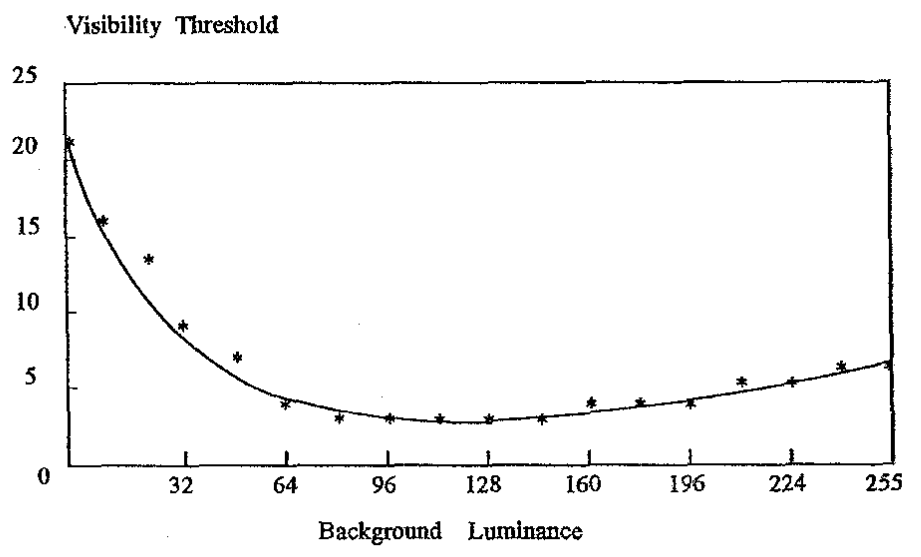
\includegraphics[width=0.66\textwidth]{bg-luma.png}
		\caption{视觉阈值与背景亮度相关曲线\cite{chun-hsienchouPerceptuallyTunedSubband1995}}
		\label{fig:bg-luma}
	\end{figure}

  \paragraph{亮度适应性} 如\ref{sec:HVS}小节,根据背景亮度的差异,人类视觉系统会调节不同的视觉敏感度,称为亮度自适应特性(Luminance Adaptation, LA)。文献\cite{chun-hsienchouPerceptuallyTunedSubband1995}表明,人眼的视觉阈值与背景亮度呈非线性关系,其关系如图\ref{fig:bg-luma}所示,当背景亮度低于127时,视觉可见性阈值以幂函数形式下降,在8位编码亮度下,当背景亮度高于127时,视觉可见性阈值随背景亮度的增加线性增长。据此,将亮度适应性与视觉阈值的关系建模为基于背景亮度的分段函数\cite{chun-hsienchouPerceptuallyTunedSubband1995},如式\ref{equ:la}所示:

  \begin{equation} \label{equ:la}
    LA(i, j) = \begin{cases}
      \left(1 - \sqrt{\frac{B(i, j)}{127}}\right) \cdot 17, &\mathrm{if}\: B(i, j)\leq 127, \\
      \left(B(i, j) - 127\right) \cdot \frac{3}{128} + 3, &\mathrm{else},
    \end{cases}
  \end{equation}
  其中,$B(i, j)$为图像中像素点$(i, j)$周围$5\times 5$范围内的亮度与图\ref{fig:5x5luma-kernel}所示的卷积核相关结果。

  \begin{figure}
    \hspace{1cm}
		\subcaptionbox{$5\times 5$背景亮度卷积核\label{fig:5x5luma-kernel}}[0.3\textwidth]{
			\begin{tabular}{|c|c|c|c|c|}	\hline
				1 & 1 & 1 & 1 & 1 \\ \hline
				1 & 2 & 2 & 2 & 1 \\ \hline
				1 & 2 & 0 & 2 & 1 \\ \hline
				1 & 2 & 2 & 2 & 1 \\ \hline
				1 & 1 & 1 & 1 & 1 \\ \hline
			\end{tabular}
    }
    \hspace{2cm}
    \subcaptionbox{$8\times 8$背景亮度卷积核\label{fig:8x8luma-kernel}}[0.3\textwidth]{
			\begin{tabular}{|c|c|c|c|c|c|c|c|}	\hline
				1& 2& 2& 3& 3& 2& 2& 1 \\ \hline
				1& 2& 0& 3& 3& 0& 2& 1 \\ \hline
				1& 3& 3& 5& 5& 3& 3& 1 \\ \hline
				1& 3& 3& 5& 5& 3& 3& 1 \\ \hline
				1& 2& 0& 3& 3& 0& 2& 1 \\ \hline
				1& 2& 2& 3& 3& 2& 2& 1 \\ \hline
				1& 1& 1& 2& 2& 1& 1& 1 \\ \hline
			\end{tabular}
		}
    \caption{背景亮度卷积核}
	\end{figure}

  \paragraph{对比度掩蔽效应} 对比度掩蔽效应是一种常见且重要掩蔽效应,指观看对比度不同的区域时产生的掩蔽效应,相比低对比度的区域,高对比度的区域具有更强的视觉掩蔽效应。根据文献\cite{wuPatternMaskingEstimation2013},对比度掩蔽效应(Constast Masking, CM)可以建模关于亮度对比度的非线性函数,由此得到对比度掩蔽效应因子$CM$,如式\ref{equ:cm}所示:

  \begin{equation} \label{equ:cm}
    CM(i, j) = 0.115 \cdot \frac{\alpha \cdot L_c(i, j)^{2.4}}{L_c(i, j)^2 + \beta^2},
  \end{equation}
  其中$\alpha$和$\beta$为常数,分别取16和26。$L_c(i, j)$为图像中像素点$(i, j)$位置的$5\times 5$范围亮度标准差。
  % question: CM到底如Matlab中的是亮度方差(标准差)还是如黄yc的论文里面写的用梯度、Prewitt算子算的。

  \paragraph{非线性组合模型} 计算得到亮度适应性因子$LA$和对比度掩蔽效应因子$CM$这两种视觉特性强度后,如何有效将它们集成在一起获得准确的JND阈值成为了一个重要问题。考虑到与只存在一种掩蔽效应相比,多个掩蔽效应会导致目标区域的失真更难以察觉,因此多个掩蔽效应的组合应采取某种形式的加法,一方面,两个掩蔽因子之间重叠会导致各自的增益降低,另一方面,需要考虑两个因子之间相互重叠的影响范围。基于以上的考虑,文献\cite{yangJustNoticeableDistortion2005}提出了一种非线性组合模型,能够将两种视觉特性强度进行组合,得到最终的JND感知阈值模型。因此,采用该非线性组合模型对亮度适应性因子$LA$和对比度掩蔽效应因子$CM$组合,得到的JND感知阈值模型,如式\ref{equ:jnd}:

  \begin{equation} \label{equ:jnd}
    \mathrm{JND}(i, j) = LA(i, j) + CM(i, j) - 0.3 \cdot \min \left\{LA(i, j) , CM(i, j)\right\}.
  \end{equation}



	\subsection{块级JND模型的提出\label{sec:blk-based-jnd}}
	原始的JND感知阈值模型是像素级模型,处理一个视频帧时,需要对其中的每个像素位置进行计算,运算量较大,严重影响算法的延迟,为了将JND感知阈值模型用在实时的低延迟编码中,需要对模型进行简化。结合后续将JND感知阈值用于分区决策中提前终止算法,将原始的像素级JND感知阈值模型简化为$8\times 8$块级模型,最小处理单位化为$8\times 8$块。式\ref{equ:la}中的亮度均值计算使用的卷积核替换为图\ref{fig:8x8luma-kernel}所示的$8\times 8$卷集合,式\ref{equ:cm}中使用的亮度标准差替换为$8\times 8$块内的亮度标准差。由此计算块级的JND感知阈值$\mathrm{JND_{8x8}}(i, j)$。

	\begin{equation} \label{equ:jnd2}
		\mathrm{JND_{8x8}}(m, n) = LA(m, n) + CM(m, n) - 0.3 \cdot \min \left\{LA(m, n) , CM(m, n)\right\},
	\end{equation}
	其中,$m, n$分别表示视频帧的$8\times 8$块行、列索引。

  根据式\ref{equ:jnd2},可以计算得到视频帧的块级JND感知阈值矩阵。其中的JND感知阈值越高,表示该$8\times 8$块的纹理细节丰富,元素排列无序,掩蔽效应较强,人类视觉系统对其失真的敏感度较低。反之,若JND感知阈值越小,表示该$8\times 8$块较为平坦,元素趋于同质,掩蔽效应较弱,人类视觉系统对失真的敏感度较高。综上,可以根据计算得到的JND感知阈值对视频帧的纹理复杂度与图像失真敏感度进行评估。

\section{JND模型计算的向量加速}
	块级JND模型的提出大大减小了JND模型的计算量,为了进一步加速JND模型的计算,对背景亮度和亮度方差使用SIMD方法进行向量加速。
	\subsection{向量加速介绍}
	单指令多数据(Single instruction, multiple data, SIMD)是一个指令同时应用于多个数据的并行化形式。当对多个数据对象执行完全相同的操作时,SIMD指令可以大大提高性能。典型的应用是数字信号处理和图形处理。下图展示了使用SIMD时单个指令可以完成未使用SIMD时需要多个指令的任务。

	\begin{figure}[!hbtp]
		\centering
		\subcaptionbox{不使用SIMD}
		[0.45\textwidth]{\resizebox{0.45\textwidth}{!}{	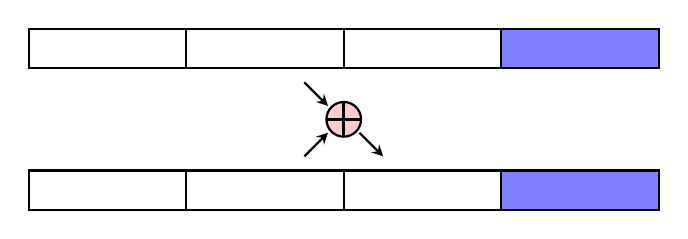
\begin{tikzpicture}

	\draw[thick] (0,0) rectangle +(2,0.5);
	\draw[thick] (2,0) rectangle +(2,0.5);
	\draw[thick] (4,0) rectangle +(2,0.5);
	\fill[blue!50] (6,0) rectangle +(2,0.5);
	\draw[thick] (6,0) rectangle +(2,0.5);
	
	\draw[-stealth, thick] (3.5,-0.18) -- (3.8,-0.48);
	\draw[-stealth, thick] (3.5,-1.12) -- (3.8,-0.82);
	\draw[stealth-, thick] (4.5,-1.12) -- (4.2,-0.82);
	
	\fill[red!20] (4,-0.65) circle (0.22cm);
	\draw[thick] (4,-0.65) circle (0.22cm);
	\draw[very thick] (3.78,-0.65) -- (4.22, -0.65);
	\draw[very thick] (4,-0.87) -- (4, -0.43);
	
	\draw[thick] (0,-1.8) rectangle +(2,0.5);
	\draw[thick] (2,-1.8) rectangle +(2,0.5);
	\draw[thick] (4,-1.8) rectangle +(2,0.5);
	\fill[blue!50] (6,-1.8) rectangle +(2,0.5);
	\draw[thick] (6,-1.8) rectangle +(2,0.5);
	\end{tikzpicture}}\label{fig:simd1}}
		\hspace{0.7cm}
		\subcaptionbox{使用SIMD}
		[0.45\textwidth]{\resizebox{0.45\textwidth}{!}{	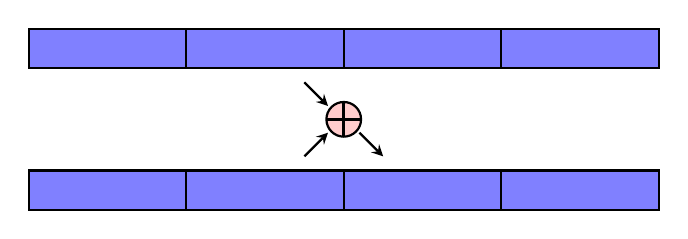
\begin{tikzpicture}

	\fill[blue!50] (0,0) rectangle +(8,0.5);
	\draw[thick] (0,0) rectangle +(2,0.5);
	\draw[thick] (2,0) rectangle +(2,0.5);
	\draw[thick] (4,0) rectangle +(2,0.5);
	\draw[thick] (6,0) rectangle +(2,0.5);
	
	\draw[-stealth, thick] (3.5,-0.18) -- (3.8,-0.48);
	\draw[-stealth, thick] (3.5,-1.12) -- (3.8,-0.82);
	\draw[stealth-, thick] (4.5,-1.12) -- (4.2,-0.82);
	
	\fill[red!20] (4,-0.65) circle (0.22cm);
	\draw[thick] (4,-0.65) circle (0.22cm);
	\draw[very thick] (3.78,-0.65) -- (4.22, -0.65);
	\draw[very thick] (4,-0.87) -- (4, -0.43);
	
	\fill[blue!50] (0,-1.8) rectangle +(8,0.5);
	\draw[thick] (0,-1.8) rectangle +(2,0.5);
	\draw[thick] (2,-1.8) rectangle +(2,0.5);
	\draw[thick] (4,-1.8) rectangle +(2,0.5);
	\draw[thick] (6,-1.8) rectangle +(2,0.5);
	\end{tikzpicture}}\label{fig:simd2}}
		\caption{SIMD操作示意图}
		\label{fig:simd}
	\end{figure}
	流式SIMD扩展(Streaming SIMD Extensions, SSE)是Intel的x86架构下的SIMD指令集扩展。SSE添加了八个128位寄存器用于向量指令,与前代指令集多媒体扩展(MultiMedia eXtension, MMX)仅支持整数处理相比,支持了浮点数学运算。SSE的后续版本还有SSE2、SSE3、SSSE3、SSE4、高级向量扩展(Advanced Vector Extensions, AVX)、AVX2、AVX-512。更高版本的指令集向量扩展具有更多、更长的寄存器以及更多的计算指令。
	\subsection{JND计算向量加速实验结果}
	经过测试,在原始像素级JND模型上计算单帧1080p图像所需的时间超过75ms,对于低延迟编码而言,超过75ms的额外延时是不可接受的,因此将像素级模型简化为块级模型是必要的,使用块级JND模型可以有效减少JND模型的计算量,只需3.4ms左右即可完成一帧的计算。

	为了进一步加速块级JND模型的计算,对背景亮度和亮度方差使用SIMD进行加速。使用SIMD可以拆开C代码中的循环,每次读入块中一行数据,一个指令对8个像素的亮度并行计算。应用SIMD后,相比块级JND模型的C级别代码可以再加速50\%的JND模型运算速度,只需要1.7ms就可以完成对一个1080p图像帧的计算。

	\begin{table}[!hpt]
		\renewcommand{\arraystretch}{0.9}
		\caption{1080p单帧图像的JND模型计算测试}
		\label{tab:jnd-compute}
		\centering
		\begin{tabular}{lccc} \toprule
			模型 & ASM & 时间 &时间比  \\ \midrule
			像素级JND模型 & C   & $>75$ms & 100\% \\
			块级JND模型   & C & $\sim 3.4$ms & 4.53\% \\
			块级JND模型   & SSE4 & $\sim 1.7$ms & 2.27\%\\ \bottomrule
		\end{tabular}
	\end{table}

  \section{基于JND的超级块快速划分优化算法}
  根据文献\cite{guoqingxiangImprovedAdaptiveQuantization2017},计算图像块的JND感知阈值方差可以反映图像块中的感知纹理一致性。若图像块的JND感知阈值方差较大,表示该块中纹理复杂度较高;反之,若图像块的JND感知阈值方差较小,表示该块相对平坦,纹理复杂度较低。在AV1视频编码中,超级块中的图像内容特性决定了超级块划分,一般对于纹理复杂度较高的区域,超级块划分较深,对于平坦的图像内容,超级块划分深度较浅、甚至不划分。图\ref{fig:jnd-sb}展示了一些超级块的划分结果,从左往右,超级块中纹理复杂度逐渐增加,对应的超级块划分更加深入仔细。

  \begin{figure}[!hbtp]
    \centering
    \subcaptionbox{简单纹理}
                    [0.24\textwidth]{
\includegraphics[height=2.5cm]{part_64x64_1.png}\label{fig:jnd-sb-1}}
    % \hspace{1cm}
    \subcaptionbox{稍复杂纹理}%
                    [0.24\textwidth]{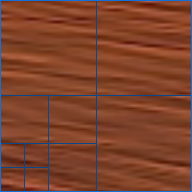
\includegraphics[height=2.5cm]{part_64x64_2.png}}
    \subcaptionbox{更复杂纹理}%
                    [0.24\textwidth]{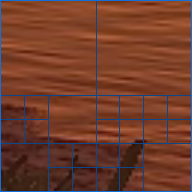
\includegraphics[height=2.5cm]{part_64x64_3.png}}
    % \hspace{1cm}
    \subcaptionbox{复杂纹理}
                    [0.24\textwidth]{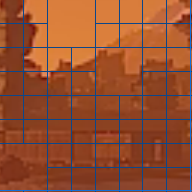
\includegraphics[height=2.5cm]{part_64x64_4.png}\label{fig:jnd-sb-4}}
    \caption{SVT-AV1超级块划分与纹理复杂度}
    \label{fig:jnd-sb}
  \end{figure}

  JND模型可以有效应用在游戏主题的直播上。游戏画面属于屏幕内容,往往是人工合成的贴图纹理,这些纹理相对自然场景视频更单调,且纹理间相似度高,单调纹理往往有高连续性。因此,在超级块划分时,游戏序列相比自然场景序列存在更多划分深度低的大块,使用基于JND的感知方法可以有效应用在游戏序列的超级块划分快速算法,下文对所提快速算法将展开具体介绍。
	\subsection{感知划分指标的提出与分析}

  根据\ref{sec:blk-based-jnd}提出的块级JND感知阈值定义,一个$8\times 8$编码块的感知特征可以通过块级的JND感知阈值$\mathrm{JND_{8x8}}(i, j)$反映,对于更高级别的编码块,其特征变化程度可以通过它的四个编码子块的JND感知阈值差异程度来表现。如式\ref{equ:pi}所示,定义一个编码块的感知划分指标PI为其四个编码子块PI的最大差值。

  \begin{equation} \label{equ:pi}
    \mathrm{PI}(d, k) =
    \begin{dcases}
      \max_{m,n\in \{0, 1, 2, 3\}} \{\mathrm{PI}(d+1, k, m) - \mathrm{PI}(d+1,k, n) \} , &\mathrm{if} \, d \leq 2,\\
      \quad \mathrm{JND_{8x8}}(k), &\mathrm{if}\, d = 2,
    \end{dcases}
  \end{equation}
  其中$d$表示划分深度,$64\times 64$划分深度为0,依次递增到$8\times 8$划分深度为3 ,$k$表示父块序号,$m, n$表示子块相对序号。PI大表明编码子块间特征差异大,更需要对其进行划分,PI小表明编码块内特征差异小,可以考虑提前终止编码块划分结构的搜索。

%  \subsubsection{感知划分指标分析}
	\begin{figure}[hbtp]
		\centering
		\subcaptionbox{64x64块划分与PI关系图}
		[0.32\textwidth]{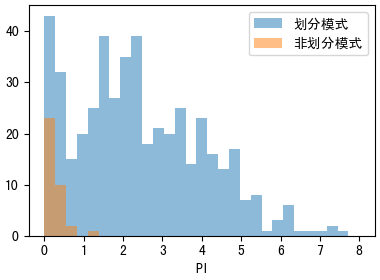
\includegraphics[width=0.325\textwidth]{pi_64.png}\label{fig:pi-64}}
		% \hspace{1cm}
		\subcaptionbox{32x32块划分与PI关系图}
		[0.32\textwidth]{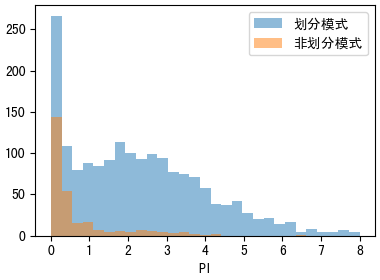
\includegraphics[width=0.325\textwidth]{pi_32.png}\label{fig:pi-32}}
		\subcaptionbox{16x16块划分与PI关系图}
		[0.32\textwidth]{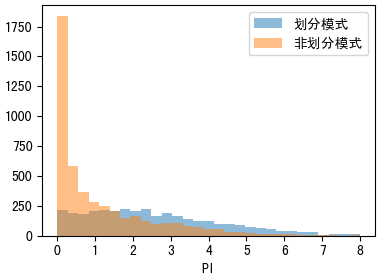
\includegraphics[width=0.325\textwidth]{pi_16.png}\label{fig:pi-16}}
		\caption{HEARTHSTONE序列划分模式与感知划分指标PI关系图(QP=31)}
		\label{fig:jnd-part-PI-example}
	\end{figure}

 使用twitch的10个1080p游戏序列分析超级块划分方式与感知划分指标PI的关系。经过测试分析,以HearthStone序列为例,其划分模式与感知划分指标PI有如图\ref{fig:jnd-part-PI-example}的关系,可以发现,非划分模式的感知划分指标PI相对较小,并且与划分模式的感知划分指标PI具有一定区分性,因此可以通过感知划分指标PI来指导块划分时的提前终止。而相对应的,划分模式的感知划分指标PI的统计特性并不能找到明显的区分性,因此通过感知划分指标PI难以指导块划分时的提前划分。造成这个区别的原因可能是一般来说游戏序列中的平坦区域比较极端化,与提前终止划分的算法契合度高,而纹理复杂区域各有各的特点,共同特性较少。


	综合分析10个1080p游戏序列,取阈值T为非划分命中率大于50\%的值来均衡加速比与bdrate的损失。另外,考虑到量化参数对块划分的影响,不同QP下应设定不同的阈值PT来提高算法性能。在较小的QP下,视频编码会分配更多的码率,通过更仔细的搜索与块划分来得到更好的重建质量,提前终止划分的感知划分指标PI的阈值PT也相对设定更小。最终的阈值T选择如表\ref{tab:av1-jnd-part-th}所示。

  \begin{table}[htbp]
    \renewcommand{\arraystretch}{0.9}
    \caption{PI提前终止划分阈值}
    \label{tab:av1-jnd-part-th}
    \centering
    \begin{tabular}{|c|c|c|c|c|c|c|c|c|} \hline
      bsize    & QP & T &bsize    & QP & T&bsize    & QP & T \\ \hline

      \multirow{4}*{$64\times 64$} & 23 & 0.09 &\multirow{4}*{$32\times 32$} & 23 & 0.30 & \multirow{4}*{$16\times 16$} & 23 & 0.40\\ \cline{2-3} \cline{5-6} \cline{8-9}
      & 31 & 0.10 & & 31 & 0.35 & & 31 & 0.45\\ \cline{2-3} \cline{5-6} \cline{8-9}
      & 39 & 0.11 & & 39 & 0.40 & & 39 & 0.50 \\ \cline{2-3} \cline{5-6} \cline{8-9}
      & 47 & 0.13 & & 47 & 0.45 & & 47 & 0.55\\ \hline
    \end{tabular}
  \end{table}

  \subsection{快速划分算法结构}

  % 介绍md_stage里面的搜索遍历结构 mds
  如前述章节\ref{sec:pd-md},SVT-AV1使用分阶段决策的方法,包括分阶段分区决策(PD)与分阶段模式选择(MD),在每个MD阶段中,会按照MD的ZigZag扫描方式递归遍历所有划分块的方式,并按照RDCOST的值比较当前块划分与非划分的花费,决策当前块是否划分。利用我们得到的感知划分指标PI,可以在当前块的PI低于一定阈值时,跳过该块的下一深度划分搜索,如\ref{fig:jnd-part-PI-alg}所示。

  \begin{figure}[!htp]
    \centering
    \resizebox{0.6\textwidth}{!}{\begin{tikzpicture}[node distance=2cm]
    \node (input) [startstop] {待划分超级块};
    \node (bsize) [decision, below of=input] {$\mathrm{bsize} \geq 16\mathrm{x}16$};
    \node (PI) [decision, below of=bsize, yshift=-0.8cm] {$\mathrm{PI} < \mathrm{PT_{bsize}}$};
    \node (skip) [process, right of=PI, xshift=3cm] {跳过下一深度划分};
    \node (RDO) [process, below of=PI, yshift=-0.6cm] {RDO};
    \node (end) [startstop, right of=RDO, xshift=3cm] {划分结束};

    %连接具体形状
    \draw [arrow](input) -- (bsize);
    \draw [arrow](bsize) -- node[left] {Yes} (PI);
    \draw [arrow](bsize) -- ($(bsize.west) + (-1.4,0)$) node[above right] {No} |- (RDO);
    \draw [arrow](PI) -- node[left] {No} (RDO);
    \draw [arrow](PI) -- node[above]{Yes} (skip);
    \draw [arrow](skip) |- (bsize);
    \draw [arrow](RDO) -- (end);

\end{tikzpicture}
}
    \caption{感知优化的超级块划分提前终止算法流程图}
    \label{fig:jnd-part-PI-alg}
  \end{figure}

  需要说明的是,因为本文对SVT-AV1的优化是基于其编码器最快预设,在最快预设下,部分AV1的特性被关闭,在块划分上,仅支持最深到$8 \times 8$的正方形划分。

  \subsection{调整md-stage进一步优化算法}
  如图\ref{fig:md}所示,SVT-AV1在每个PD阶段中包含多个模式选择MD阶段,在每个MD阶段中会使用各类预测工具与性能指标对各个候选模式进行评估,只留下性能最好的一部分候选,在下一个MD阶段中继续竞争。理论上,多MD阶段决策的最终优化目标是RDO,因为直接计算RDO的计算量较高,在前期的MD阶段中,会使用一些快速算法替代,以牺牲准确性的前提减少了计算量,在最后的MD阶段会使用完整的RDO计算每个候选的RDCOST。在前期快速算法评估下性能较好的候选在完整RDO的评估下的性能可能较差,因此每个MD阶段需要留下一定数量的候选,以防止错失最终性能较好的候选。

  基于JND感知阈值,可以对各阶段的md-stage保留数量做进一步调整以减小计算量。JND感知阈值较高的区域,人眼视觉系统对其失真的敏感度较低,可以适当减小保留的候选数量\texttt{md-stage-count},即使错过最优的候选对视觉效果的影响也比较低。

  \section{实验结果与分析\label{sec:jnd-test}}

  \subsection{实验环境配置}
  实验使用个人笔记本电脑完成,实验系统配置如表\ref{tab:os}所示,实验使用SVT-AV1配置如表\ref{tab:svt}所示,实验测试了All Intra和Low Delay P两种GoP结构,QP取$\{23, 31, 39, 47\}$(由于MINECRAFT序列在QP取值较低时的VMAF非常接近,为了得到正常的BD-Rate-VMAF,对于MINECRAFT序列取QP为$\{31, 39, 47, 55\}$)。

  \begin{table}[htbp]
		\renewcommand{\arraystretch}{0.9}
		\caption{实验系统配置}
		\label{tab:os}
		\centering
		\begin{tabular}{lc} \toprule
			项目& 参数  \\ \midrule
			OS:     &Manjaro 20.0 Lysia\\
			Kernel: & x86\_64 Linux 5.6.7-1-MANJARO\\
			CPU:    &Intel Core i7-6700HQ (8) @ 3.500GHz\\
			RAM:    &16GB\\
			GCC:    &v9.3.0\\
			SVT-AV1: & v0.8.1\\ \bottomrule
		\end{tabular}
	\end{table}
  \begin{table}[htbp]
		\renewcommand{\arraystretch}{0.9}
		\caption{SVT-AV1编码器参数配置}
		\label{tab:svt}
		\centering
		\begin{tabular}{lc} \toprule
			项目& 参数  \\ \midrule
			preset     &8\\
			pred-struct& LDP\\
			lookahead    &0\\
			fps    &60\\
			GoP    &60\\
			asm    & up tp avx2\\
			bitdepth & 8\\
			hierarchicalLevels  & 4 \\
			rc & CQP\\ \bottomrule
		\end{tabular}
	\end{table}
  编码测试结果包括比特率Bitrate,峰值信噪比(Peak Signal to Noise Ratio, PSNR),视频多方法评估融合(Video Multimethod Assessment Fusion, VMAF\cite{liPracticalPerceptualVideo}),\ref{sec:svt-profile}章节中提出的SVT-AV1框架的profile工具被用于记录编码时各模块的CPU使用时间,取ENCDEC过程的CPU时间总和作为编码时间来评估算法应用前后的编码复杂度。

  测试序列取twitch的8个1080p游戏序列,一方面游戏直播作为一大重要的直播类型,有着很高的研究价值,另一方面,游戏场景通常是屏幕内容类型的人工场景,场景中简单纹理较多,适合所提算法的测试。

  测试时使用命令\texttt{sudo cpupower frequency-set -g performance}将CPU频率策略调整为“Performance”以锁定CPU频率,以确保按照CPU使用时间计算的算法计算量对比准确。





	\subsection{实验测试质量指标}

	\paragraph{PSNR}
	峰值信噪比(Peak Signal to Noise Ratio, PSNR)表示信号的最大可能功率与影响信号保真度的噪声功率之间的比率。因为许多信号具有非常宽的动态范围,PSNR通常用对数分贝标度表示。PSNR是最常用的图像、视频客观质量评价指标,但是PSNR算法逐像素比较参考视频和失真视频,研究\cite{huynh-thuAccuracyPSNRPredicting2012}表明,由于失真的可见性在某种程度上取决于视频内容,因此PSNR无法如实表示人类对视觉失真的感知,尽管如此,PSNR仍是编解码器比较的事实上标准。

	PSNR通过均方误差(mean square error, MSE)定义,给定原始$m\times n$图像$I$与其失真图像$K$,MSE定义为:
	\begin{equation}
		\mathrm{MSE} = \frac{1}{mn} \sum_{i=0}^{m-1} \sum_{j=0}^{n-1}[I(i, j) - K(i, j)]^2.
	\end{equation}

	由此,PSNR(dB单位)定义为:
	\begin{equation}
	\mathrm{PSNR} = 10 \times \log_{10} \left(\frac{\mathrm{MAX}_I^2}{\mathrm{MSE}}\right),
	\end{equation}
	其中,$\mathrm{MAX}_I$表示原始图像的最大可能像素值。
	\paragraph{VMAF}
	视频多方法评估融合(Video Multimethod Assessment Fusion, VMAF\cite{liPracticalPerceptualVideo})是Netflix与南加州大学和德克萨斯大学奥斯汀分校的图像与视频工程实验室合作开发的客观全参考视频质量指标。它根据参考视频序列预测失真视频序列的主观视频质量。

	VMAF使用多种图像质量评价指标来预测视频质量,并使用基于支持向量机(support vector machines, SVM)的回归将多种指标融合,对每个视频帧输出$[0,100]$的分数,最后,对整个视频序列的输出分数求算术平均值得到最终的差分平均意见分数(differential mean opinion score, DMOS),VMAF使用的图像质量评价指标包括包括:
	\begin{enumerate}[label=\arabic*)]
		\item 视觉信息保真度(Visual Information Fidelity, VIF):考虑四个不同空间尺度上的信息保真度损失;
		\item 细节损失指标(Detail Loss Metric, DLM):用于衡量细节损失和损害观众注意力的障碍;
		\item 平均同位像素差异(Mean Co-Located Pixel Difference, MCPD):测量亮度分量上帧之间的时间差异;
		\item 抗噪信噪比(Anti-noise signal-to-noise ratio, AN-SNR)。
	\end{enumerate}

	文献\cite{liPracticalPerceptualVideo,barmanEvaluationVideoQuality2018a, leeComparisonObjectiveQuality2017}的测试结果表明,VMAF在多种数据集上的表现均好于其他主观评价指标,特别的,文献\cite{barmanEvaluationVideoQuality2018a}展示了对于游戏视频场景,VMAF的性能远高于其他VQA指标。

	\paragraph{BD-Rate} Bjontegaard速率差\cite{Bjontegaard2001CalculationOA}(BD-Rate)允许在保持与客观指标所测量的相同质量水平时,定量比较编解码器提供的比特率降低。速率变化计算为质量范围内速率的平均百分比差异。

  \subsection{实验结果分析}

  对算法性能的评估通过测试两种图像质量评价指标完成,分别是峰值信噪比PSNR指标和与视频多方法评估融合VMAF指标。
  对算法性能的评估分为两点:

  \begin{enumerate}[label=\arabic*)]
    \item 使用提前终止划分的快速算法带来的编码复杂度降低,通过编码时间节省比例表现;
    \item 算法导致的编码性能下降,通过比特率与峰值信噪比PSNR指标、视频多方法评估融合VMAF指标综合分析BD-Rate表现。
  \end{enumerate}

  表\ref{tab:av1-jnd-part-AI}、\ref{tab:av1-jnd-part-ldp}分别是在All Intra、Low Delay P预测结构下的实验结果,表\ref{tab:av1-jnd-part-AI-md-stage}是在All Intra预测结构加上调整md\_stage得到的实验结果。

  从实验结果有以下发现:

  \begin{enumerate}[label=\arabic*)]
    \item 对于ALL Intra和Low Delay P两种预测结构,所提算法均可以减少15\%左右的编码时间,其中All Intra的编码时间减少量略高于Low Delay P;
    \item 所提的快速算法会增加编码的码率、减小图像质量,因此BD-Rate会有一定程度的上升,其中All Intra的BD-Rate增加量少于Low Delay P;
    \item 不同游戏序列的编码时间减少量和BD-Rate增加都有所不同,这是因为不同游戏序列的画面纹理特征有较大差异,而我们使用的是一个相对一般化的感知划分指标阈值。
  \end{enumerate}

  需要注意的是,本算法以SVT-AV1编码器的最快预设为基础实现,SVT-AV1本身已经实现了一些用于块划分的快速算法。本算法的编码时间减少量与BD-Rate增加量成对抗关系,若选取更激进的感知划分指标阈值,将会以损失更多BD-Rate的代价来减少更多的编码时间;同理,若选取更保守的感知划分指标阈值,BD-Rate的增加将会减少,但在编码时间上得到的增益也会减小。


  \begin{table}[!hpt]
    \renewcommand{\arraystretch}{0.9}
    \caption{JND快速编码测试结果ALL Intra}
    \label{tab:av1-jnd-part-AI}
    \centering
    \begin{tabular}{|c|c|c|c|c|c|c|c|} \hline
      序列    & QP & $\Delta$T &  $\Delta$Bitrate & $\Delta$PSNR & $\Delta$VMAF & \makecell{BD-Rate\\(PSNR)} & \makecell{BD-Rate\\(VMAF)}\\ \hline

      \multirow{4}*{CSGO} & 23 & -24.98\% & +1.86\% & -0.10 & -0.046 & \multirow{4}*{+3.88\%} & \multirow{4}*{+4.53\%} \\ \cline{2-6}
      & 31 & -33.25\% & +1.73\% & -0.11 & -0.096 &  & \\ \cline{2-6}
      & 39 & -29.15\% & +1.65\% & -0.09 & -0.096 &  & \\ \cline{2-6}
      & 47 & -27.92\% & +1.55\% & -0.08 & -0.071 &  & \\ \hline
      \multirow{4}*{DOTA2} & 23 & -15.75\% & +0.70\% & -0.10 & -0.025 & \multirow{4}*{+1.46\%} & \multirow{4}*{+1.40\%} \\ \cline{2-6}
      & 31 & -22.29\% & +0.13\% & -0.08 & -0.054 &  & \\ \cline{2-6}
      & 39 & -16.84\% & -0.04\% & -0.06 & -0.050 &  & \\ \cline{2-6}
      & 47 & -14.33\% & +0.06\% & -0.04 & -0.044 &  & \\ \hline
      \multirow{4}*{EuroTruckSim2} & 23 & -13.45\% & +0.20\% & -0.20 & -0.000 & \multirow{4}*{+1.43\%} & \multirow{4}*{-2.46\%} \\ \cline{2-6}
      & 31 & -17.37\% & +0.02\% & -0.11 & -0.007 &  & \\ \cline{2-6}
      & 39 & -9.68\% & -0.05\% & -0.07 & -0.049 &  & \\ \cline{2-6}
      & 47 & -9.42\% & -0.03\% & -0.05 & -0.042 &  & \\ \hline
      \multirow{4}*{FALLOUT4} & 23 & -13.42\% & +0.55\% & -0.05 & -0.011 & \multirow{4}*{+0.91\%} & \multirow{4}*{+0.99\%} \\ \cline{2-6}
      & 31 & -13.43\% & +0.23\% & -0.05 & -0.014 &  & \\ \cline{2-6}
      & 39 & -10.32\% & +0.11\% & -0.04 & -0.022 &  & \\ \cline{2-6}
      & 47 & -12.82\% & +0.06\% & -0.03 & -0.024 &  & \\ \hline
      \multirow{4}*{GTAV} & 23 & -4.51\% & +0.13\% & -0.05 & -0.016 & \multirow{4}*{+0.55\%} & \multirow{4}*{+0.70\%} \\ \cline{2-6}
      & 31 & -21.02\% & +0.05\% & -0.03 & -0.020 &  & \\ \cline{2-6}
      & 39 & -9.55\% & -0.01\% & -0.03 & -0.031 &  & \\ \cline{2-6}
      & 47 & -16.22\% & -0.02\% & -0.02 & -0.037 &  & \\ \hline
      \multirow{4}*{HEARTHSTONE} & 23 & -20.03\% & +0.10\% & -0.01 & -0.000 & \multirow{4}*{+0.29\%} & \multirow{4}*{+0.26\%} \\ \cline{2-6}
      & 31 & -17.56\% & +0.04\% & -0.02 & -0.009 &  & \\ \cline{2-6}
      & 39 & -17.02\% & +0.04\% & -0.02 & -0.008 &  & \\ \cline{2-6}
      & 47 & -9.94\% & +0.01\% & -0.02 & -0.012 &  & \\ \hline
      \multirow{4}*{MINECRAFT} & 23 & -4.90\% & +0.71\% & -0.11 & -0.001 & \multirow{4}*{+1.09\%} & \multirow{4}*{-0.34\%} \\ \cline{2-6}
      & 31 & -9.00\% & +0.40\% & -0.09 & -0.001 &  & \\ \cline{2-6}
      & 39 & -8.78\% & +0.18\% & -0.07 & -0.006 &  & \\ \cline{2-6}
      & 47 & -11.04\% & +0.08\% & -0.05 & -0.001 &  & \\ \hline
      \multirow{4}*{RUST} & 23 & -25.32\% & -0.57\% & -0.28 & -0.032 & \multirow{4}*{+1.70\%} & \multirow{4}*{+1.86\%} \\ \cline{2-6}
      & 31 & -24.67\% & +0.06\% & -0.12 & -0.080 &  & \\ \cline{2-6}
      & 39 & -25.06\% & -0.08\% & -0.10 & -0.135 &  & \\ \cline{2-6}
      & 47 & -21.98\% & -0.20\% & -0.07 & -0.147 &  & \\ \hline
      \multirow{4}*{STARCRAFT} & 23 & -9.29\% & +1.69\% & -0.10 & -0.000 & \multirow{4}*{+2.15\%} & \multirow{4}*{+10.79\%} \\ \cline{2-6}
      & 31 & -14.63\% & +0.98\% & -0.11 & -0.000 &  & \\ \cline{2-6}
      & 39 & -13.79\% & +0.59\% & -0.09 & -0.005 &  & \\ \cline{2-6}
      & 47 & -15.10\% & +0.47\% & -0.06 & -0.016 &  & \\ \hline
      \multirow{4}*{WITCHER3} & 23 & -20.09\% & +0.77\% & -0.21 & -0.053 & \multirow{4}*{+2.82\%} & \multirow{4}*{+3.63\%} \\ \cline{2-6}
      & 31 & -22.96\% & +0.34\% & -0.15 & -0.144 &  & \\ \cline{2-6}
      & 39 & -25.36\% & -0.22\% & -0.14 & -0.207 &  & \\ \cline{2-6}
      & 47 & -23.16\% & -0.36\% & -0.10 & -0.209 &  & \\ \hline
      \multicolumn{2}{|c|}{平均值} & -16.89\% & +0.35\% & -0.08 & -0.046 & +1.63\% & +2.14\%

      \\\hline
    \end{tabular}
  \end{table}

  \begin{table}[!hpt]
    \renewcommand{\arraystretch}{0.9}
    \caption{JND快速编码测试结果Low Delay P}
    \label{tab:av1-jnd-part-ldp}
    \centering
    \begin{tabular}{|c|c|c|c|c|c|c|c|} \hline
      序列    & QP & $\Delta$T &  $\Delta$Bitrate & $\Delta$PSNR & $\Delta$VMAF & \makecell{BD-Rate\\(PSNR)} & \makecell{BD-Rate\\(VMAF)}\\ \hline

      \multirow{4}*{CSGO} & 23 & -24.59\% & -0.17\% & -0.13 & -0.001 & \multirow{4}*{+3.12\%} & \multirow{4}*{+2.41\%} \\ \cline{2-6}
      & 31 & -26.33\% & +0.80\% & -0.08 & -0.001 &  & \\ \cline{2-6}
      & 39 & -19.99\% & +1.35\% & -0.07 & -0.001 &  & \\ \cline{2-6}
      & 47 & -26.84\% & +1.90\% & -0.05 & -0.001 &  & \\ \hline
      \multirow{4}*{DOTA2} & 23 & -13.68\% & +0.97\% & -0.09 & -0.001 & \multirow{4}*{+2.37\%} & \multirow{4}*{+2.39\%} \\ \cline{2-6}
      & 31 & -14.37\% & +0.25\% & -0.07 & -0.000 &  & \\ \cline{2-6}
      & 39 & -16.17\% & -0.01\% & -0.05 & -0.001 &  & \\ \cline{2-6}
      & 47 & -16.77\% & -0.03\% & -0.04 & -0.001 &  & \\ \hline
      \multirow{4}*{EuroTruckSim2} & 23 & -7.95\% & +0.45\% & -0.05 & -0.000 & \multirow{4}*{+1.53\%} & \multirow{4}*{+2.03\%} \\ \cline{2-6}
      & 31 & -6.41\% & +0.29\% & -0.06 & -0.001 &  & \\ \cline{2-6}
      & 39 & -7.82\% & +0.21\% & -0.06 & -0.002 &  & \\ \cline{2-6}
      & 47 & -10.69\% & +0.16\% & -0.03 & -0.001 &  & \\ \hline
      \multirow{4}*{FALLOUT4} & 23 & -5.75\% & +0.35\% & -0.04 & -0.000 & \multirow{4}*{+1.09\%} & \multirow{4}*{+1.33\%} \\ \cline{2-6}
      & 31 & -8.01\% & +0.23\% & -0.03 & -0.001 &  & \\ \cline{2-6}
      & 39 & -9.70\% & +0.07\% & -0.03 & -0.001 &  & \\ \cline{2-6}
      & 47 & -10.98\% & +0.25\% & -0.02 & -0.001 &  & \\ \hline
      \multirow{4}*{GTAV} & 23 & -8.56\% & +0.75\% & -0.04 & -0.000 & \multirow{4}*{+2.32\%} & \multirow{4}*{+2.17\%} \\ \cline{2-6}
      & 31 & -11.10\% & +1.15\% & -0.05 & -0.001 &  & \\ \cline{2-6}
      & 39 & -10.55\% & +0.38\% & -0.03 & -0.001 &  & \\ \cline{2-6}
      & 47 & -10.16\% & +0.12\% & -0.04 & -0.002 &  & \\ \hline
      \multirow{4}*{HEARTHSTONE} & 23 & -10.97\% & -0.52\% & -0.03 & -0.000 & \multirow{4}*{+0.42\%} & \multirow{4}*{+0.96\%} \\ \cline{2-6}
      & 31 & -10.41\% & +0.21\% & -0.01 & -0.000 &  & \\ \cline{2-6}
      & 39 & -10.33\% & +0.25\% & -0.02 & -0.000 &  & \\ \cline{2-6}
      & 47 & -9.43\% & +0.07\% & -0.02 & -0.000 &  & \\ \hline
      \multirow{4}*{MINECRAFT} & 31 & -4.16\% & +0.24\% & -0.06 & -0.000 & \multirow{4}*{+1.02\%} & \multirow{4}*{-0.13\%} \\ \cline{2-6}
      & 39 & -5.86\% & +0.30\% & -0.04 & -0.001 &  & \\ \cline{2-6}
      & 47 & -6.91\% & -0.16\% & -0.04 & -0.002 &  & \\ \cline{2-6}
      & 55 & -10.36\% & -0.35\% & -0.02 & -0.002 &  & \\ \hline
      \multirow{4}*{RUST} & 23 & -15.99\% & +0.89\% & -0.10 & -0.001 & \multirow{4}*{+3.03\%} & \multirow{4}*{+2.57\%} \\ \cline{2-6}
      & 31 & -17.93\% & +1.31\% & -0.06 & -0.002 &  & \\ \cline{2-6}
      & 39 & -17.50\% & +0.14\% & -0.07 & -0.002 &  & \\ \cline{2-6}
      & 47 & -20.22\% & -0.62\% & -0.06 & -0.003 &  & \\ \hline
      \multirow{4}*{STARCRAFT} & 23 & -9.06\% & +1.17\% & -0.06 & -0.000 & \multirow{4}*{+1.72\%} & \multirow{4}*{-3.21\%} \\ \cline{2-6}
      & 31 & -9.53\% & +0.71\% & -0.06 & -0.000 &  & \\ \cline{2-6}
      & 39 & -9.31\% & +0.20\% & -0.06 & -0.001 &  & \\ \cline{2-6}
      & 47 & -9.76\% & +0.52\% & -0.03 & -0.001 &  & \\ \hline
      \multirow{4}*{WITCHER3} & 23 & -18.55\% & +0.42\% & -0.12 & -0.002 & \multirow{4}*{+3.82\%} & \multirow{4}*{+2.59\%} \\ \cline{2-6}
      & 31 & -21.62\% & +0.04\% & -0.12 & -0.003 &  & \\ \cline{2-6}
      & 39 & -17.42\% & -0.70\% & -0.09 & -0.003 &  & \\ \cline{2-6}
      & 47 & -20.60\% & -1.18\% & -0.04 & -0.002 &  & \\ \hline
      \multicolumn{2}{|c|}{平均值} & -13.06\% & +0.31\% & -0.05 & -0.001 & +2.04\% & +1.31\%

       \\\hline
    \end{tabular}
  \end{table}

  \begin{table}[!hpt]
    \renewcommand{\arraystretch}{0.9}
    \caption{调整md-stage进一步优化JND快速编码测试结果All Intra}
    \label{tab:av1-jnd-part-AI-md-stage}
    \centering
    \begin{tabular}{|c|c|c|c|c|c|c|c|} \hline
      序列    & QP & $\Delta$T &  $\Delta$Bitrate & $\Delta$PSNR & $\Delta$VMAF & \makecell{BD-Rate\\(PSNR)} & \makecell{BD-Rate\\(VMAF)}\\ \hline

      \multirow{4}*{CSGO} & 23 & -49.01\% & +2.23\% & -0.13 & -0.048 & \multirow{4}*{+4.78\%} & \multirow{4}*{+5.19\%} \\ \cline{2-6}
      & 31 & -46.94\% & +1.86\% & -0.13 & -0.103 &  & \\ \cline{2-6}
      & 39 & -44.36\% & +1.88\% & -0.13 & -0.117 &  & \\ \cline{2-6}
      & 47 & -40.54\% & +1.99\% & -0.12 & -0.102 &  & \\ \hline
      \multirow{4}*{DOTA2} & 23 & -35.24\% & +0.91\% & -0.11 & -0.018 & \multirow{4}*{+1.87\%} & \multirow{4}*{+1.80\%} \\ \cline{2-6}
      & 31 & -38.34\% & +0.32\% & -0.09 & -0.059 &  & \\ \cline{2-6}
      & 39 & -30.65\% & +0.03\% & -0.09 & -0.072 &  & \\ \cline{2-6}
      & 47 & -31.13\% & +0.18\% & -0.06 & -0.058 &  & \\ \hline
      \multirow{4}*{EuroTruckSim2} & 23 & -36.84\% & +0.31\% & -0.23 & -0.001 & \multirow{4}*{+1.81\%} & \multirow{4}*{-2.55\%} \\ \cline{2-6}
      & 31 & -34.28\% & +0.14\% & -0.13 & -0.009 &  & \\ \cline{2-6}
      & 39 & -27.65\% & -0.05\% & -0.09 & -0.069 &  & \\ \cline{2-6}
      & 47 & -27.67\% & -0.06\% & -0.07 & -0.074 &  & \\ \hline
      \multirow{4}*{FALLOUT4} & 23 & -29.81\% & +0.89\% & -0.07 & -0.010 & \multirow{4}*{+1.53\%} & \multirow{4}*{+1.57\%} \\ \cline{2-6}
      & 31 & -29.64\% & +0.50\% & -0.07 & -0.017 &  & \\ \cline{2-6}
      & 39 & -22.24\% & +0.38\% & -0.07 & -0.028 &  & \\ \cline{2-6}
      & 47 & -23.67\% & +0.34\% & -0.06 & -0.056 &  & \\ \hline
      \multirow{4}*{GTAV} & 23 & -28.42\% & +0.30\% & -0.07 & -0.016 & \multirow{4}*{+1.04\%} & \multirow{4}*{+1.27\%} \\ \cline{2-6}
      & 31 & -32.79\% & +0.07\% & -0.06 & -0.035 &  & \\ \cline{2-6}
      & 39 & -26.01\% & -0.03\% & -0.06 & -0.061 &  & \\ \cline{2-6}
      & 47 & -31.04\% & -0.03\% & -0.05 & -0.082 &  & \\ \hline
      \multirow{4}*{HEARTHSTONE} & 23 & -35.88\% & +0.41\% & -0.03 & -0.004 & \multirow{4}*{+0.81\%} & \multirow{4}*{+0.72\%} \\ \cline{2-6}
      & 31 & -31.95\% & +0.24\% & -0.05 & -0.008 &  & \\ \cline{2-6}
      & 39 & -27.62\% & +0.24\% & -0.05 & -0.031 &  & \\ \cline{2-6}
      & 47 & -25.36\% & +0.22\% & -0.04 & -0.030 &  & \\ \hline
      \multirow{4}*{MINECRAFT} & 23 & -25.34\% & +0.68\% & -0.13 & -0.001 & \multirow{4}*{+1.17\%} & \multirow{4}*{+0.43\%} \\ \cline{2-6}
      & 31 & -25.46\% & +0.26\% & -0.11 & -0.000 &  & \\ \cline{2-6}
      & 39 & -23.94\% & +0.08\% & -0.09 & -0.009 &  & \\ \cline{2-6}
      & 47 & -25.77\% & +0.05\% & -0.06 & -0.004 &  & \\ \hline
      \multirow{4}*{RUST} & 23 & -40.12\% & -0.31\% & -0.32 & -0.018 & \multirow{4}*{+2.04\%} & \multirow{4}*{+1.99\%} \\ \cline{2-6}
      & 31 & -37.87\% & +0.04\% & -0.15 & -0.083 &  & \\ \cline{2-6}
      & 39 & -37.09\% & -0.17\% & -0.12 & -0.159 &  & \\ \cline{2-6}
      & 47 & -33.71\% & -0.35\% & -0.09 & -0.161 &  & \\ \hline
      \multirow{4}*{STARCRAFT} & 23 & -30.98\% & +1.85\% & -0.12 & -0.000 & \multirow{4}*{+2.50\%} & \multirow{4}*{+5.58\%} \\ \cline{2-6}
      & 31 & -29.00\% & +1.09\% & -0.12 & -0.001 &  & \\ \cline{2-6}
      & 39 & -30.69\% & +0.72\% & -0.11 & -0.006 &  & \\ \cline{2-6}
      & 47 & -29.44\% & +0.64\% & -0.08 & -0.015 &  & \\ \hline
      \multirow{4}*{WITCHER3} & 23 & -38.68\% & +0.74\% & -0.23 & -0.053 & \multirow{4}*{+2.97\%} & \multirow{4}*{+4.24\%} \\ \cline{2-6}
      & 31 & -40.61\% & +0.22\% & -0.16 & -0.174 &  & \\ \cline{2-6}
      & 39 & -39.68\% & -0.38\% & -0.15 & -0.243 &  & \\ \cline{2-6}
      & 47 & -37.01\% & -0.60\% & -0.12 & -0.305 &  & \\ \hline
      \multicolumn{2}{|c|}{平均值} & -32.81\% & +0.45\% & -0.11 & -0.058 & +2.05\% & +2.02\%

       \\\hline
    \end{tabular}
  \end{table}
\vspace{-10pt}
  \subsubsection{实验结果主观评估}

  图\ref{fig:dota2-part}展示了在DOTA2序列上,原始算法与所提算法的超级块划分对比图,其中图\ref{fig:dota2-origin-part}展示了SVT-AV1原始算法的超级块划分,图\ref{fig:dota2-jnd-part}展示了应用基于JND的快速划分算法后的超级块划分效果,图\ref{fig:dota2-md-part}展示了基于JND调整md-stage的快速划分算法后的超级块划分效果。对比发现,在纹理简单、一致性较高的区域,应用了所提算法后,更倾向于划分较大的块;对于纹理复杂的区域,二者的划分比较一致,均有细致的分块。

  \begin{figure}[!hbtp]
    \setlength\abovecaptionskip{-0.05cm}
    \centering
    \subcaptionbox{原始算法超级块划分图\label{fig:dota2-origin-part}}
                    [\textwidth]{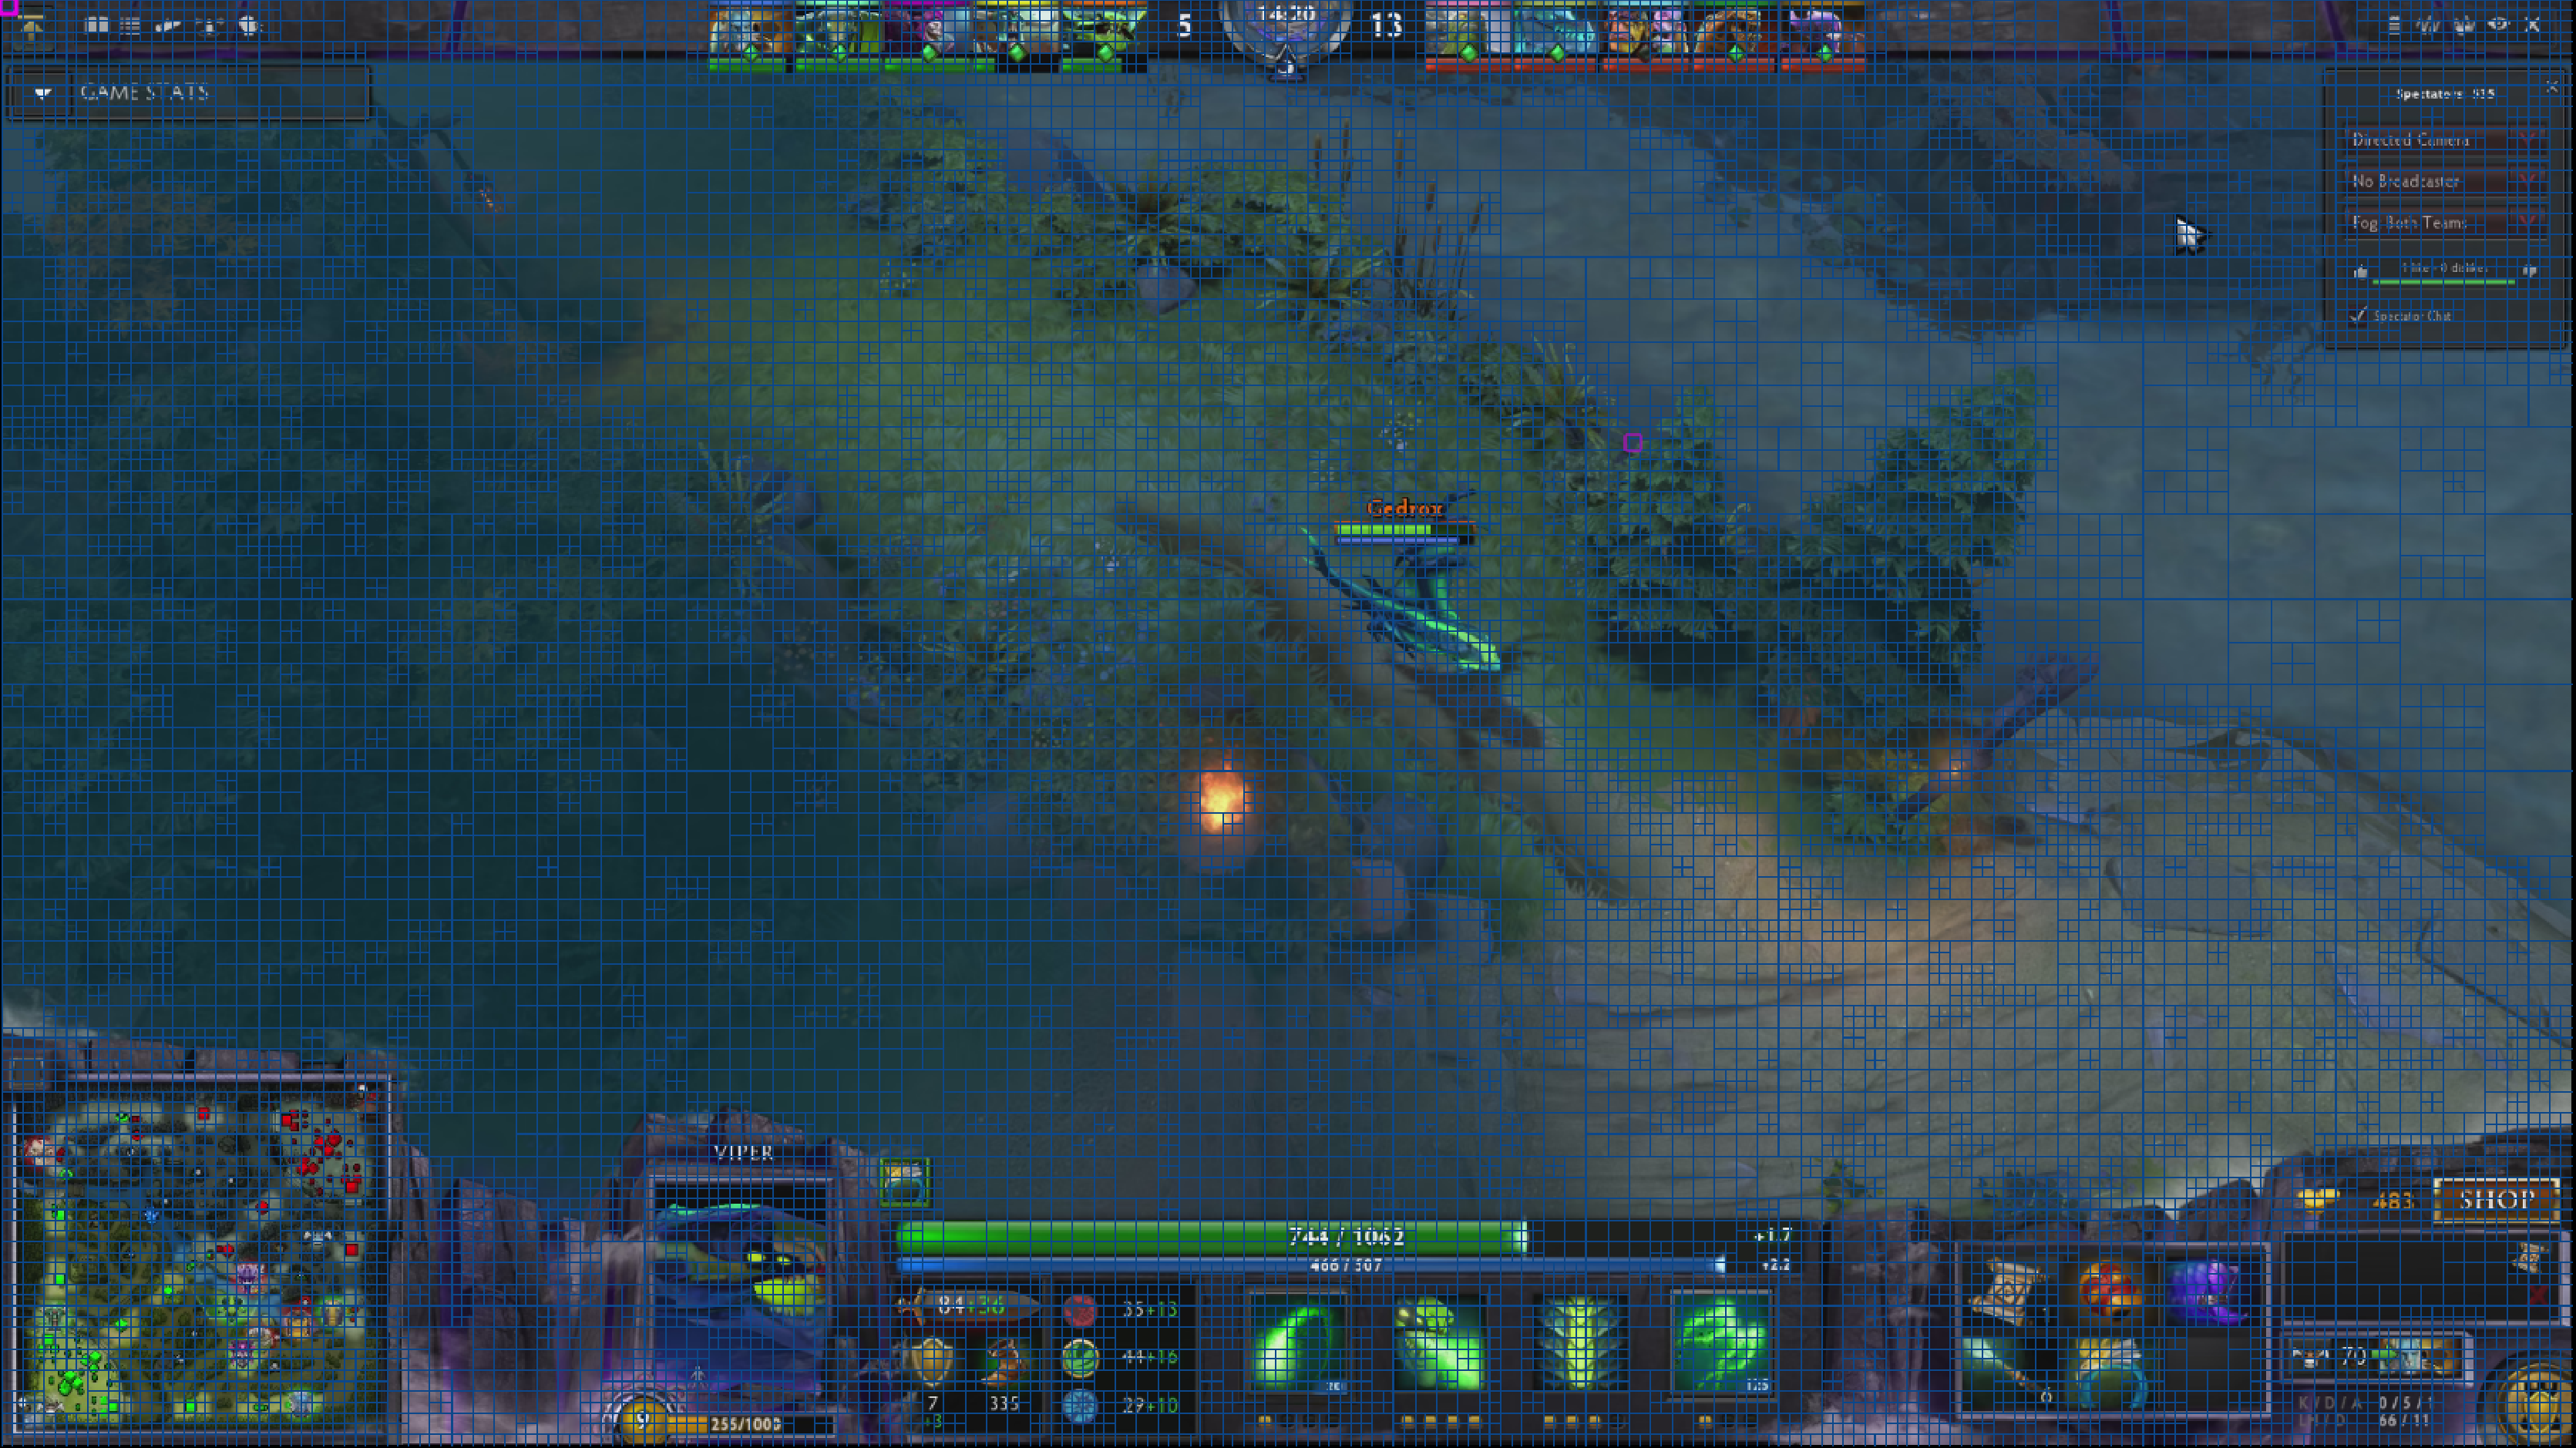
\includegraphics[width=0.885\textwidth]{dota2_origin_partition.pdf}}
    \subcaptionbox{JND优化快速算法超级块划分图\label{fig:dota2-jnd-part}}
                    [\textwidth]{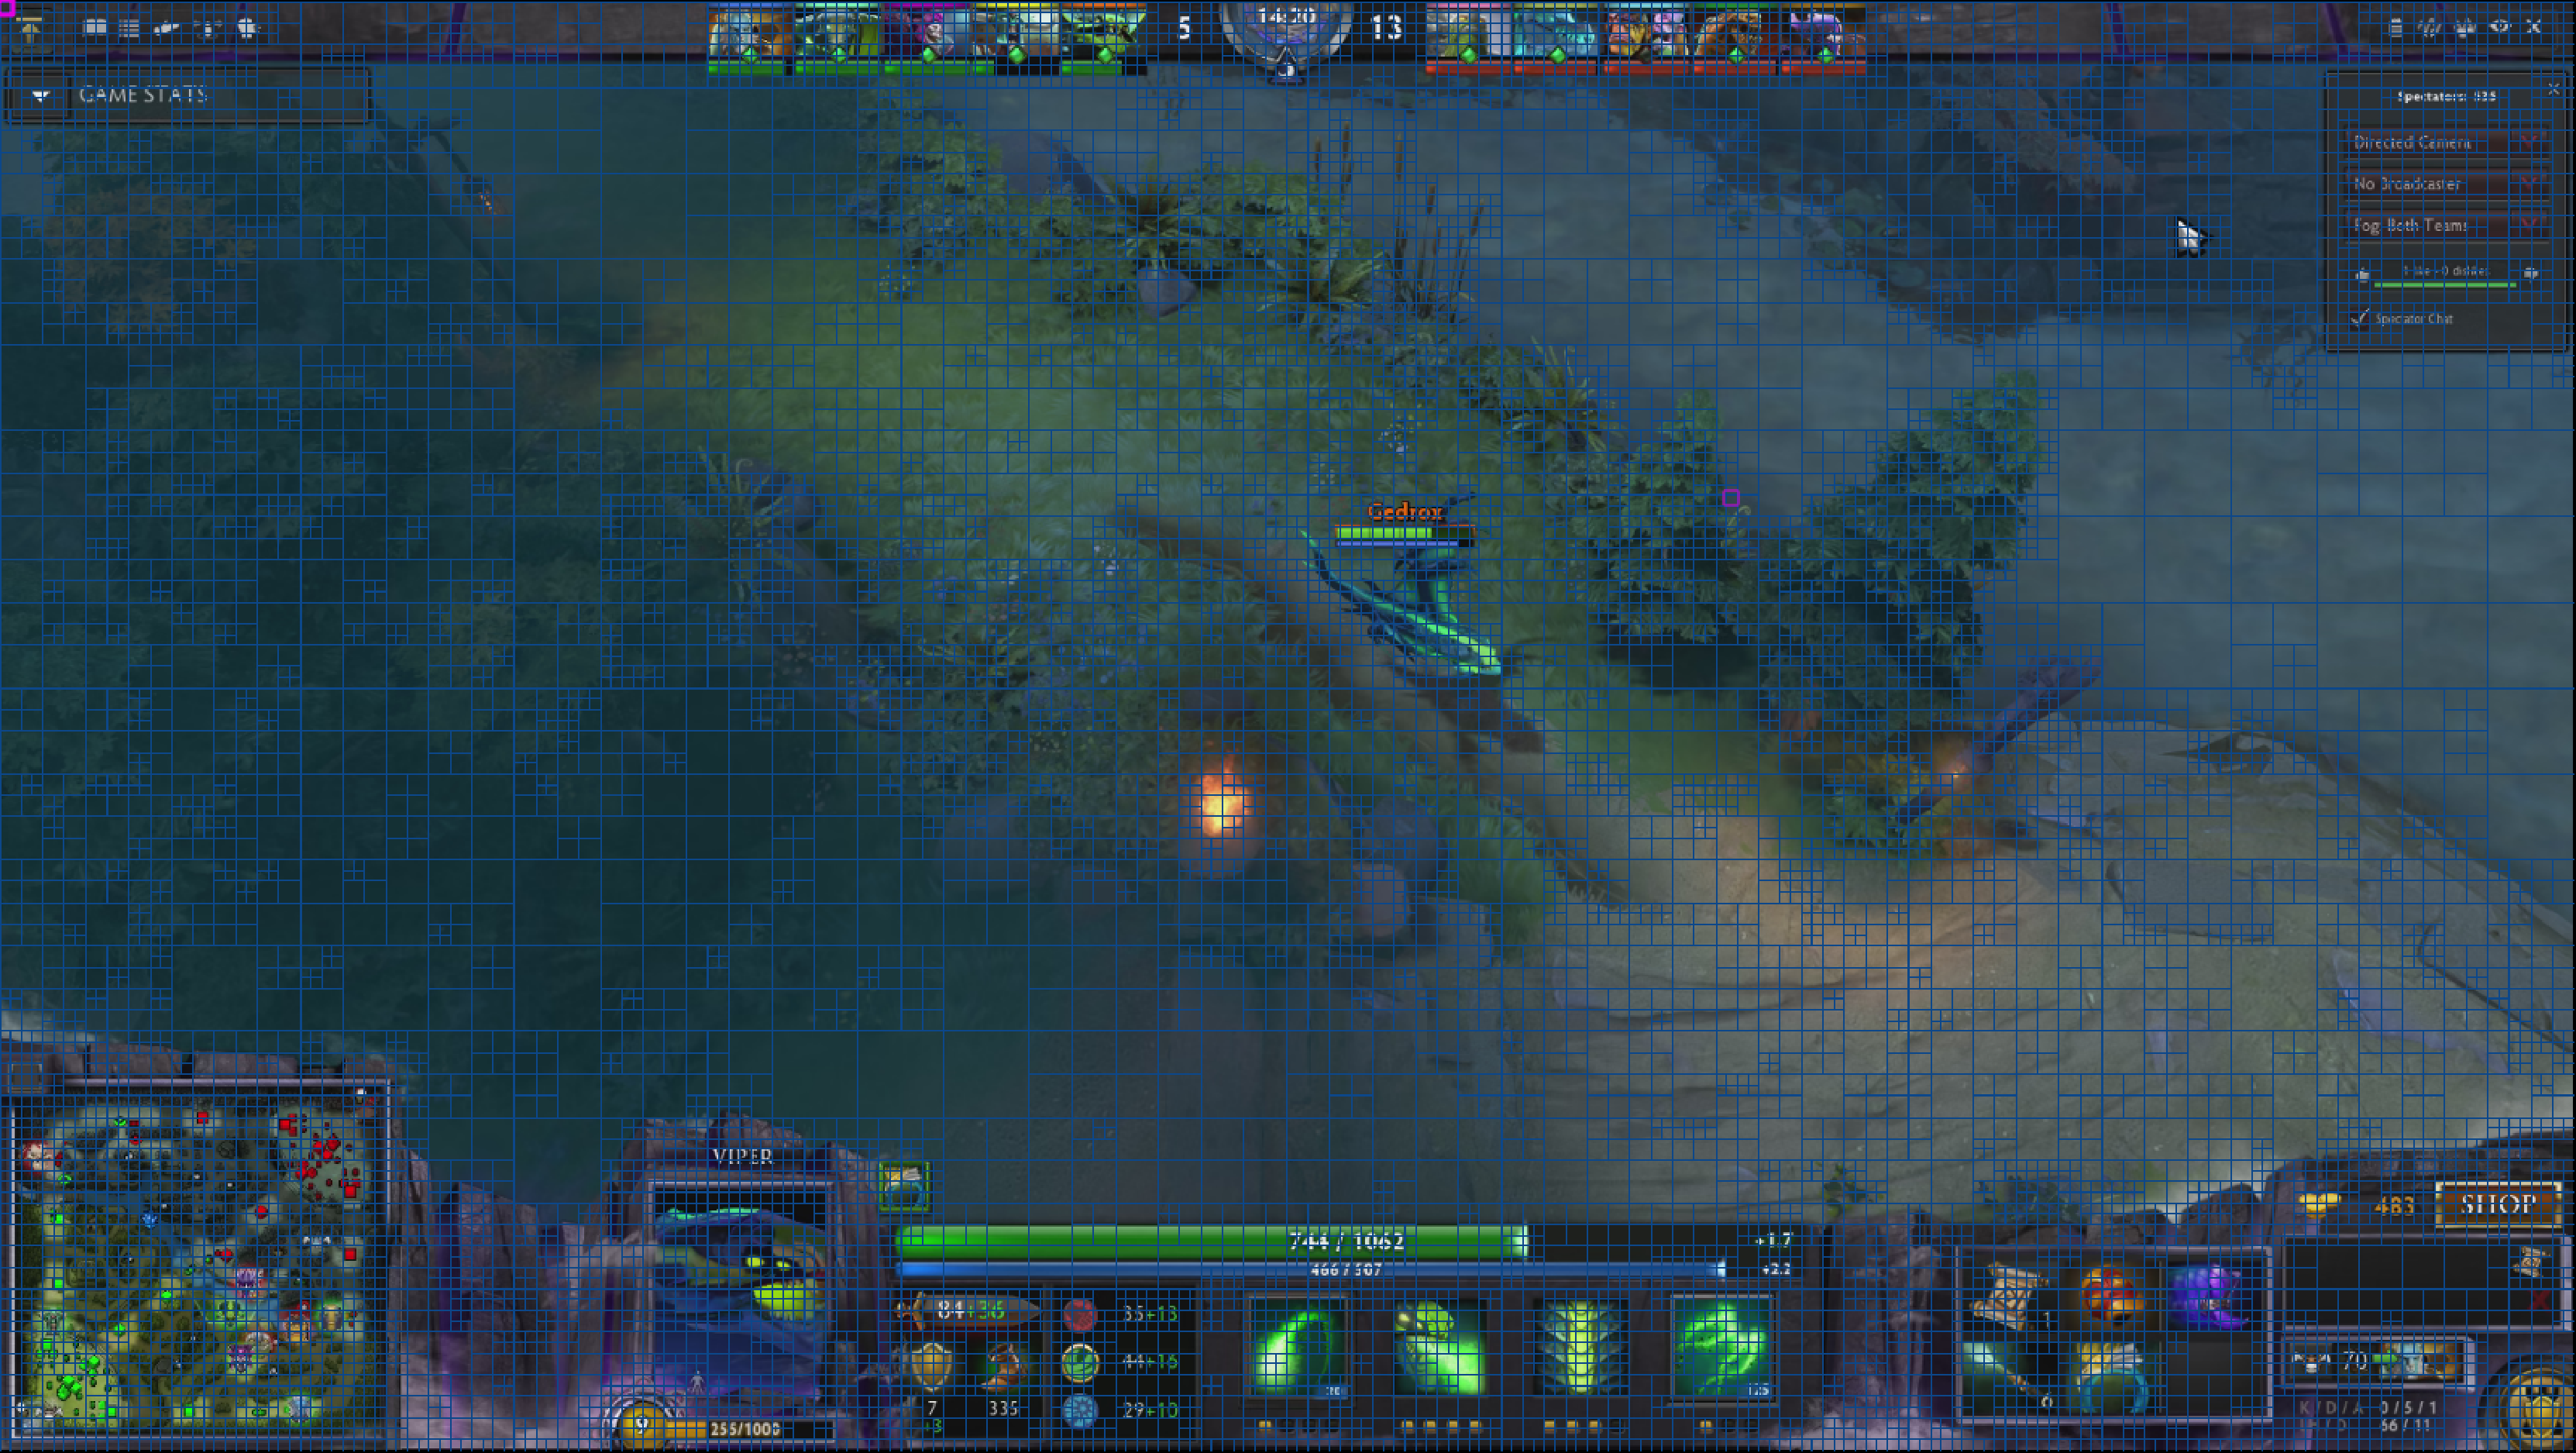
\includegraphics[width=0.885\textwidth]{dota2_jnd_partition.pdf}}
    \subcaptionbox{md-stage调整的JND优化快速算法超级块划分图\label{fig:dota2-md-part}}
                    [\textwidth]{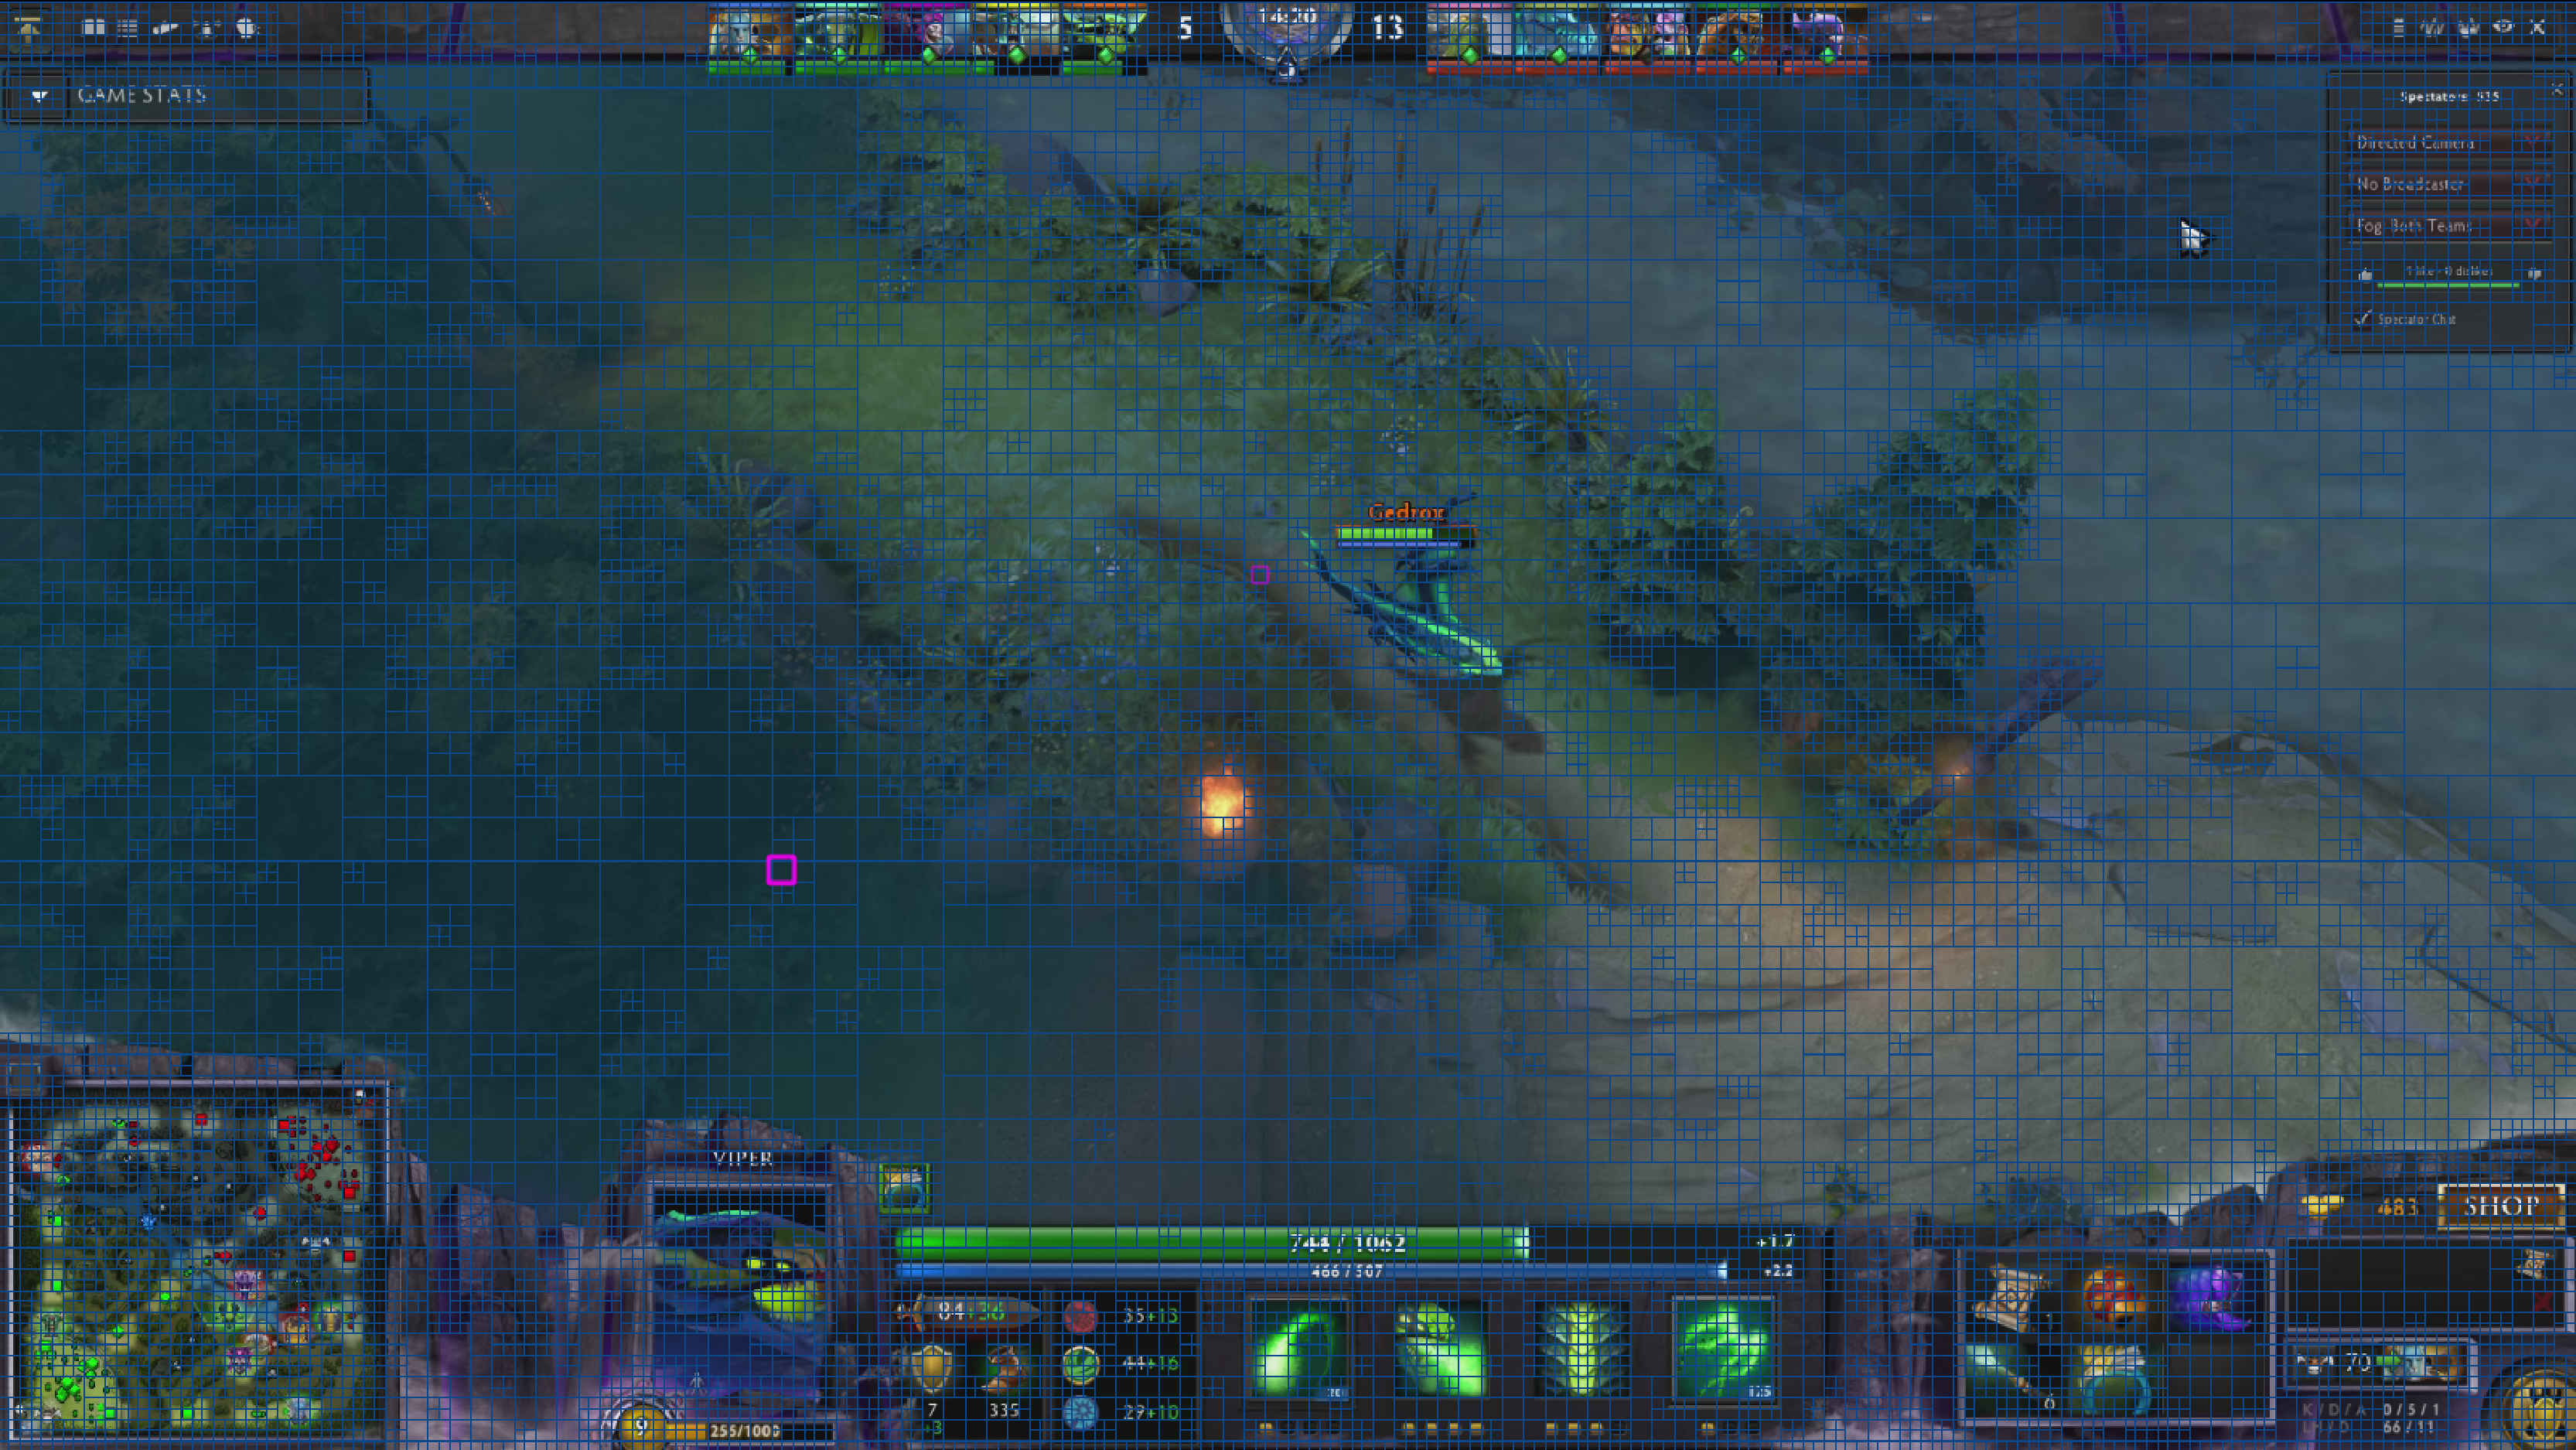
\includegraphics[width=0.885\textwidth]{dota2_md_partition.pdf}}
    \caption{原始算法与所提算法的超级块划分对比图}
    \label{fig:dota2-part}
  \end{figure}

  图\ref{fig:dota2-decode}展示了在DOTA2序列上,原始算法与所提算法的解码图像对比,其中图\ref{fig:dota2-origin-dec}展示了SVT-AV1原始算法的解码图像,图\ref{fig:dota2-jnd-dec}展示了应用基于JND的快速划分算法后的解码图像,图\ref{fig:dota2-md-dec}展示了应用基于JND调整md-stage的快速划分算法后的解码图像。对比发现,使用所提算法对主观质量基本没有影响。

  \begin{figure}[!hbtp]
    \setlength\abovecaptionskip{-0.05cm}
    \centering
    \subcaptionbox{原始算法解码图像\label{fig:dota2-origin-dec}}
                    [\textwidth]{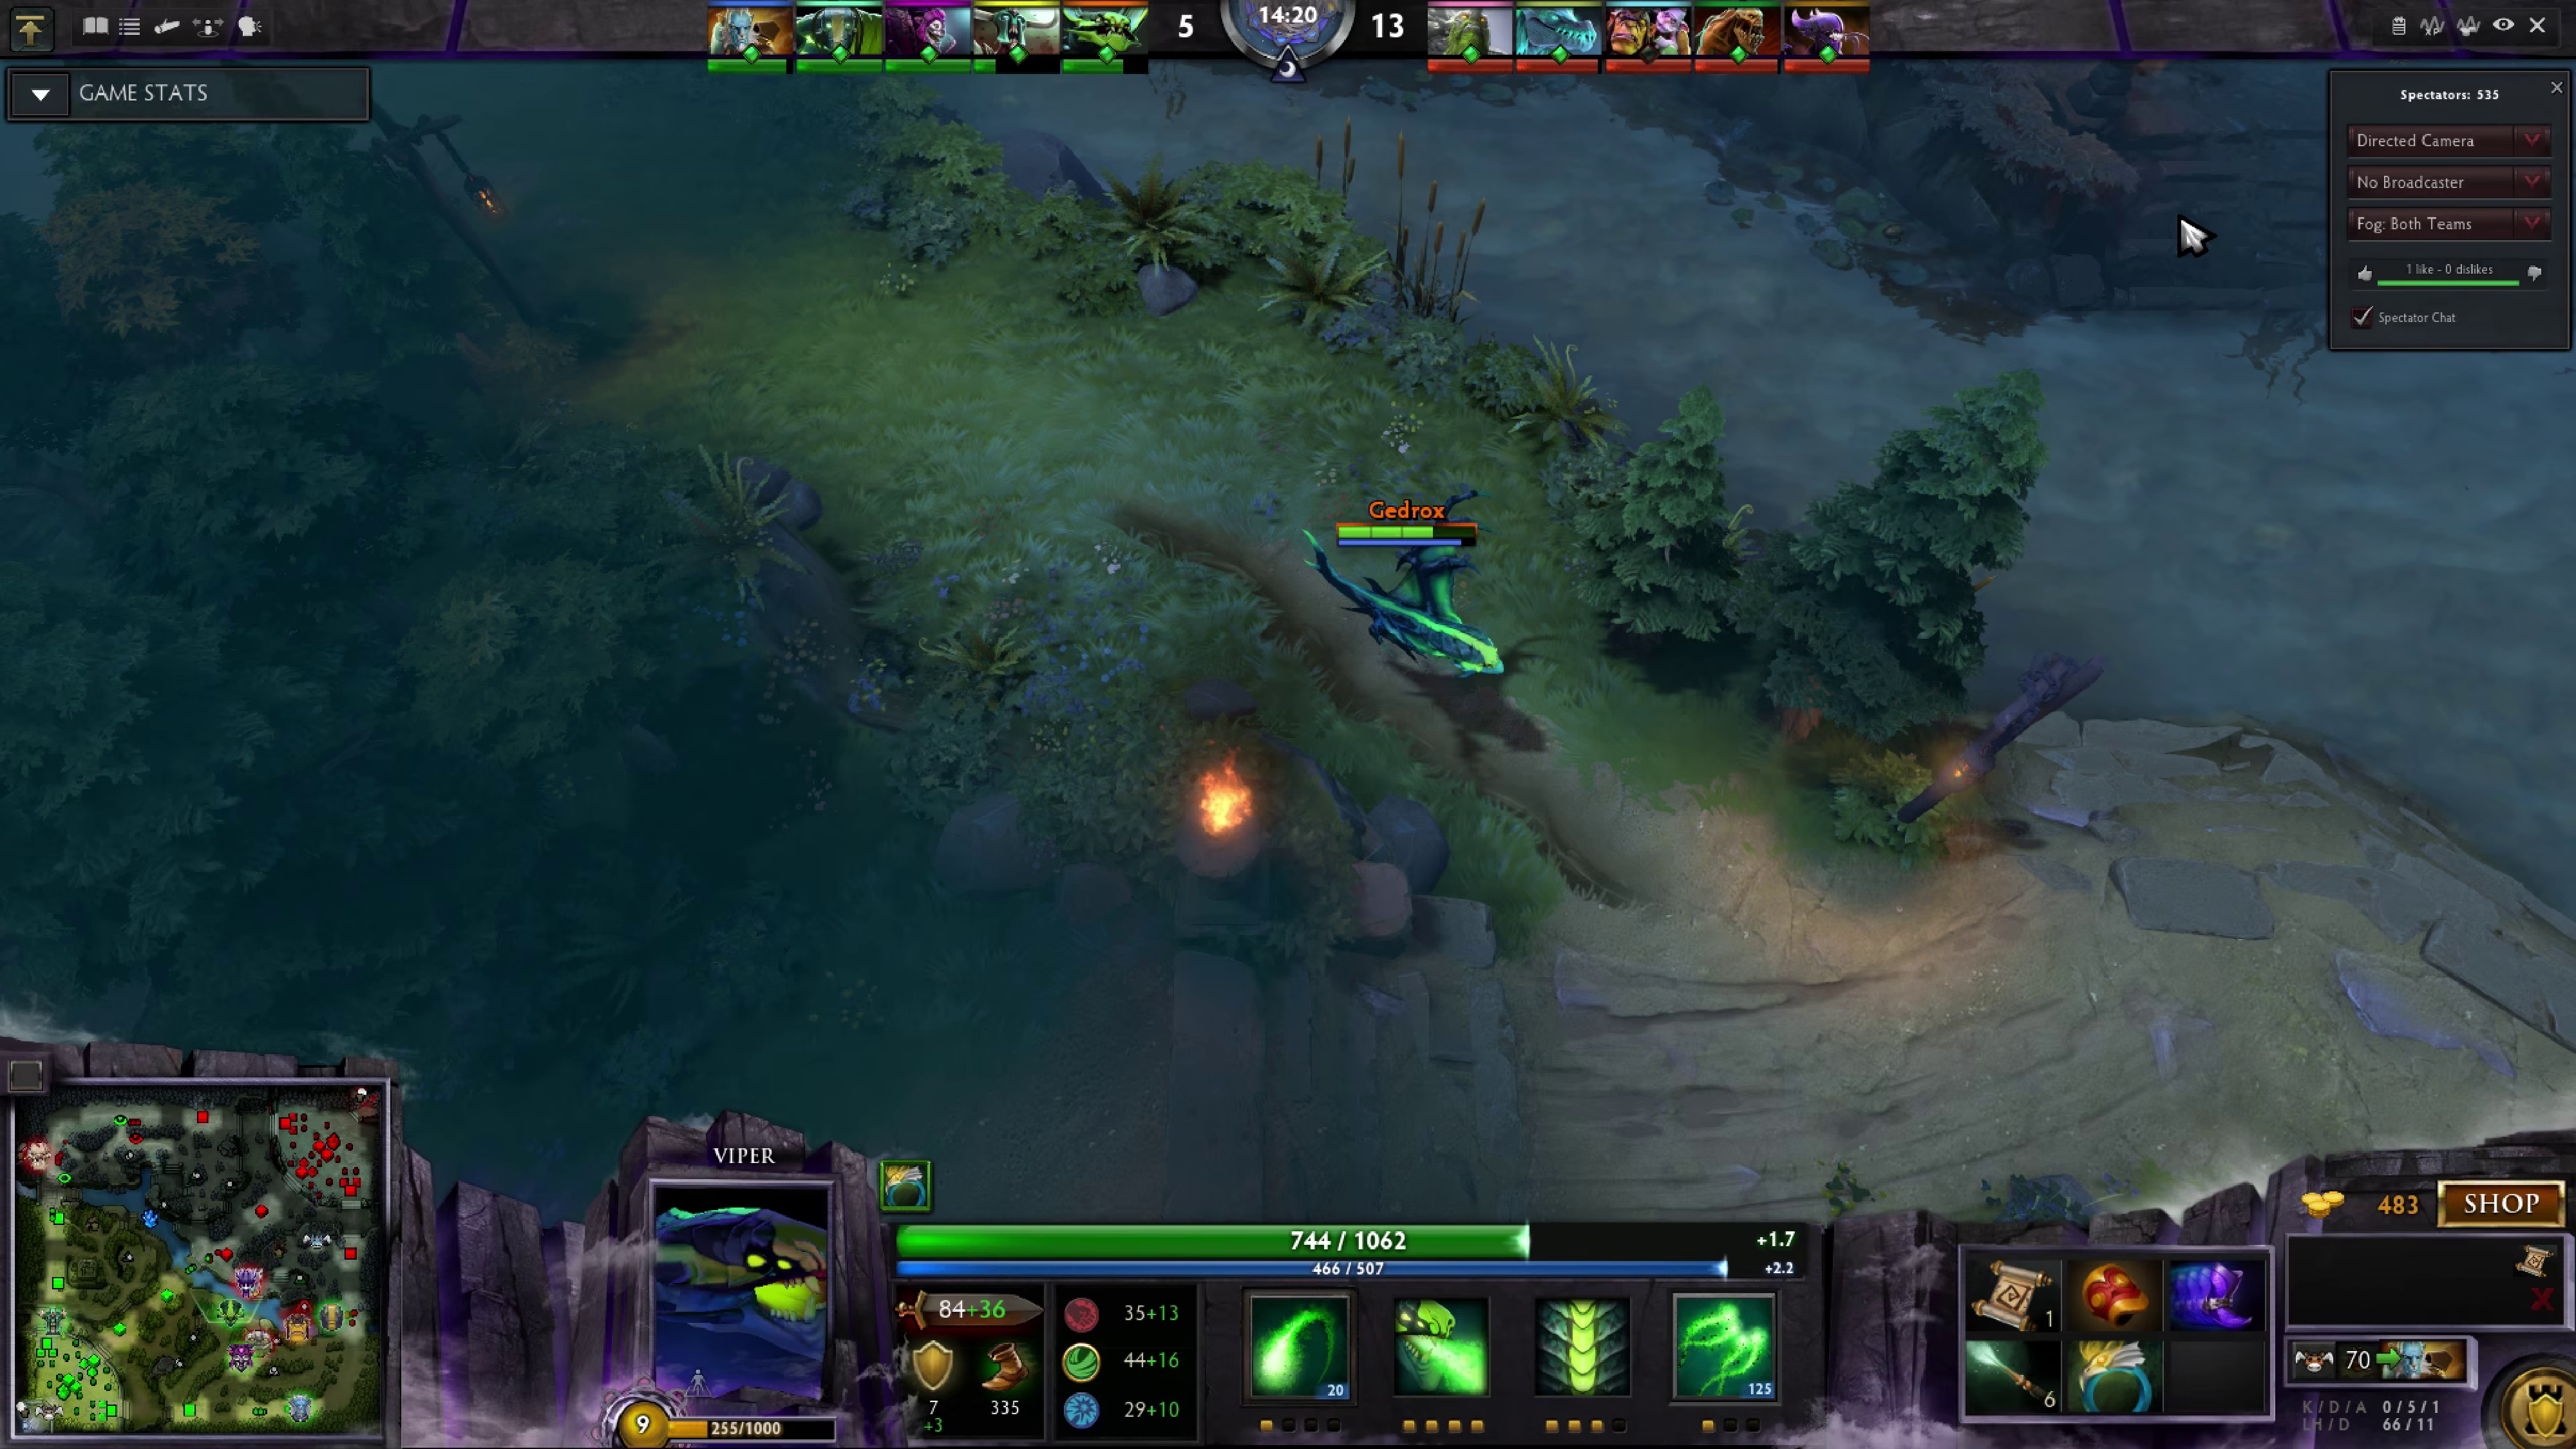
\includegraphics[width=0.885\textwidth]{dota2_origin_decode.pdf}}
    \subcaptionbox{所提算法解码图像\label{fig:dota2-jnd-dec}}
                    [\textwidth]{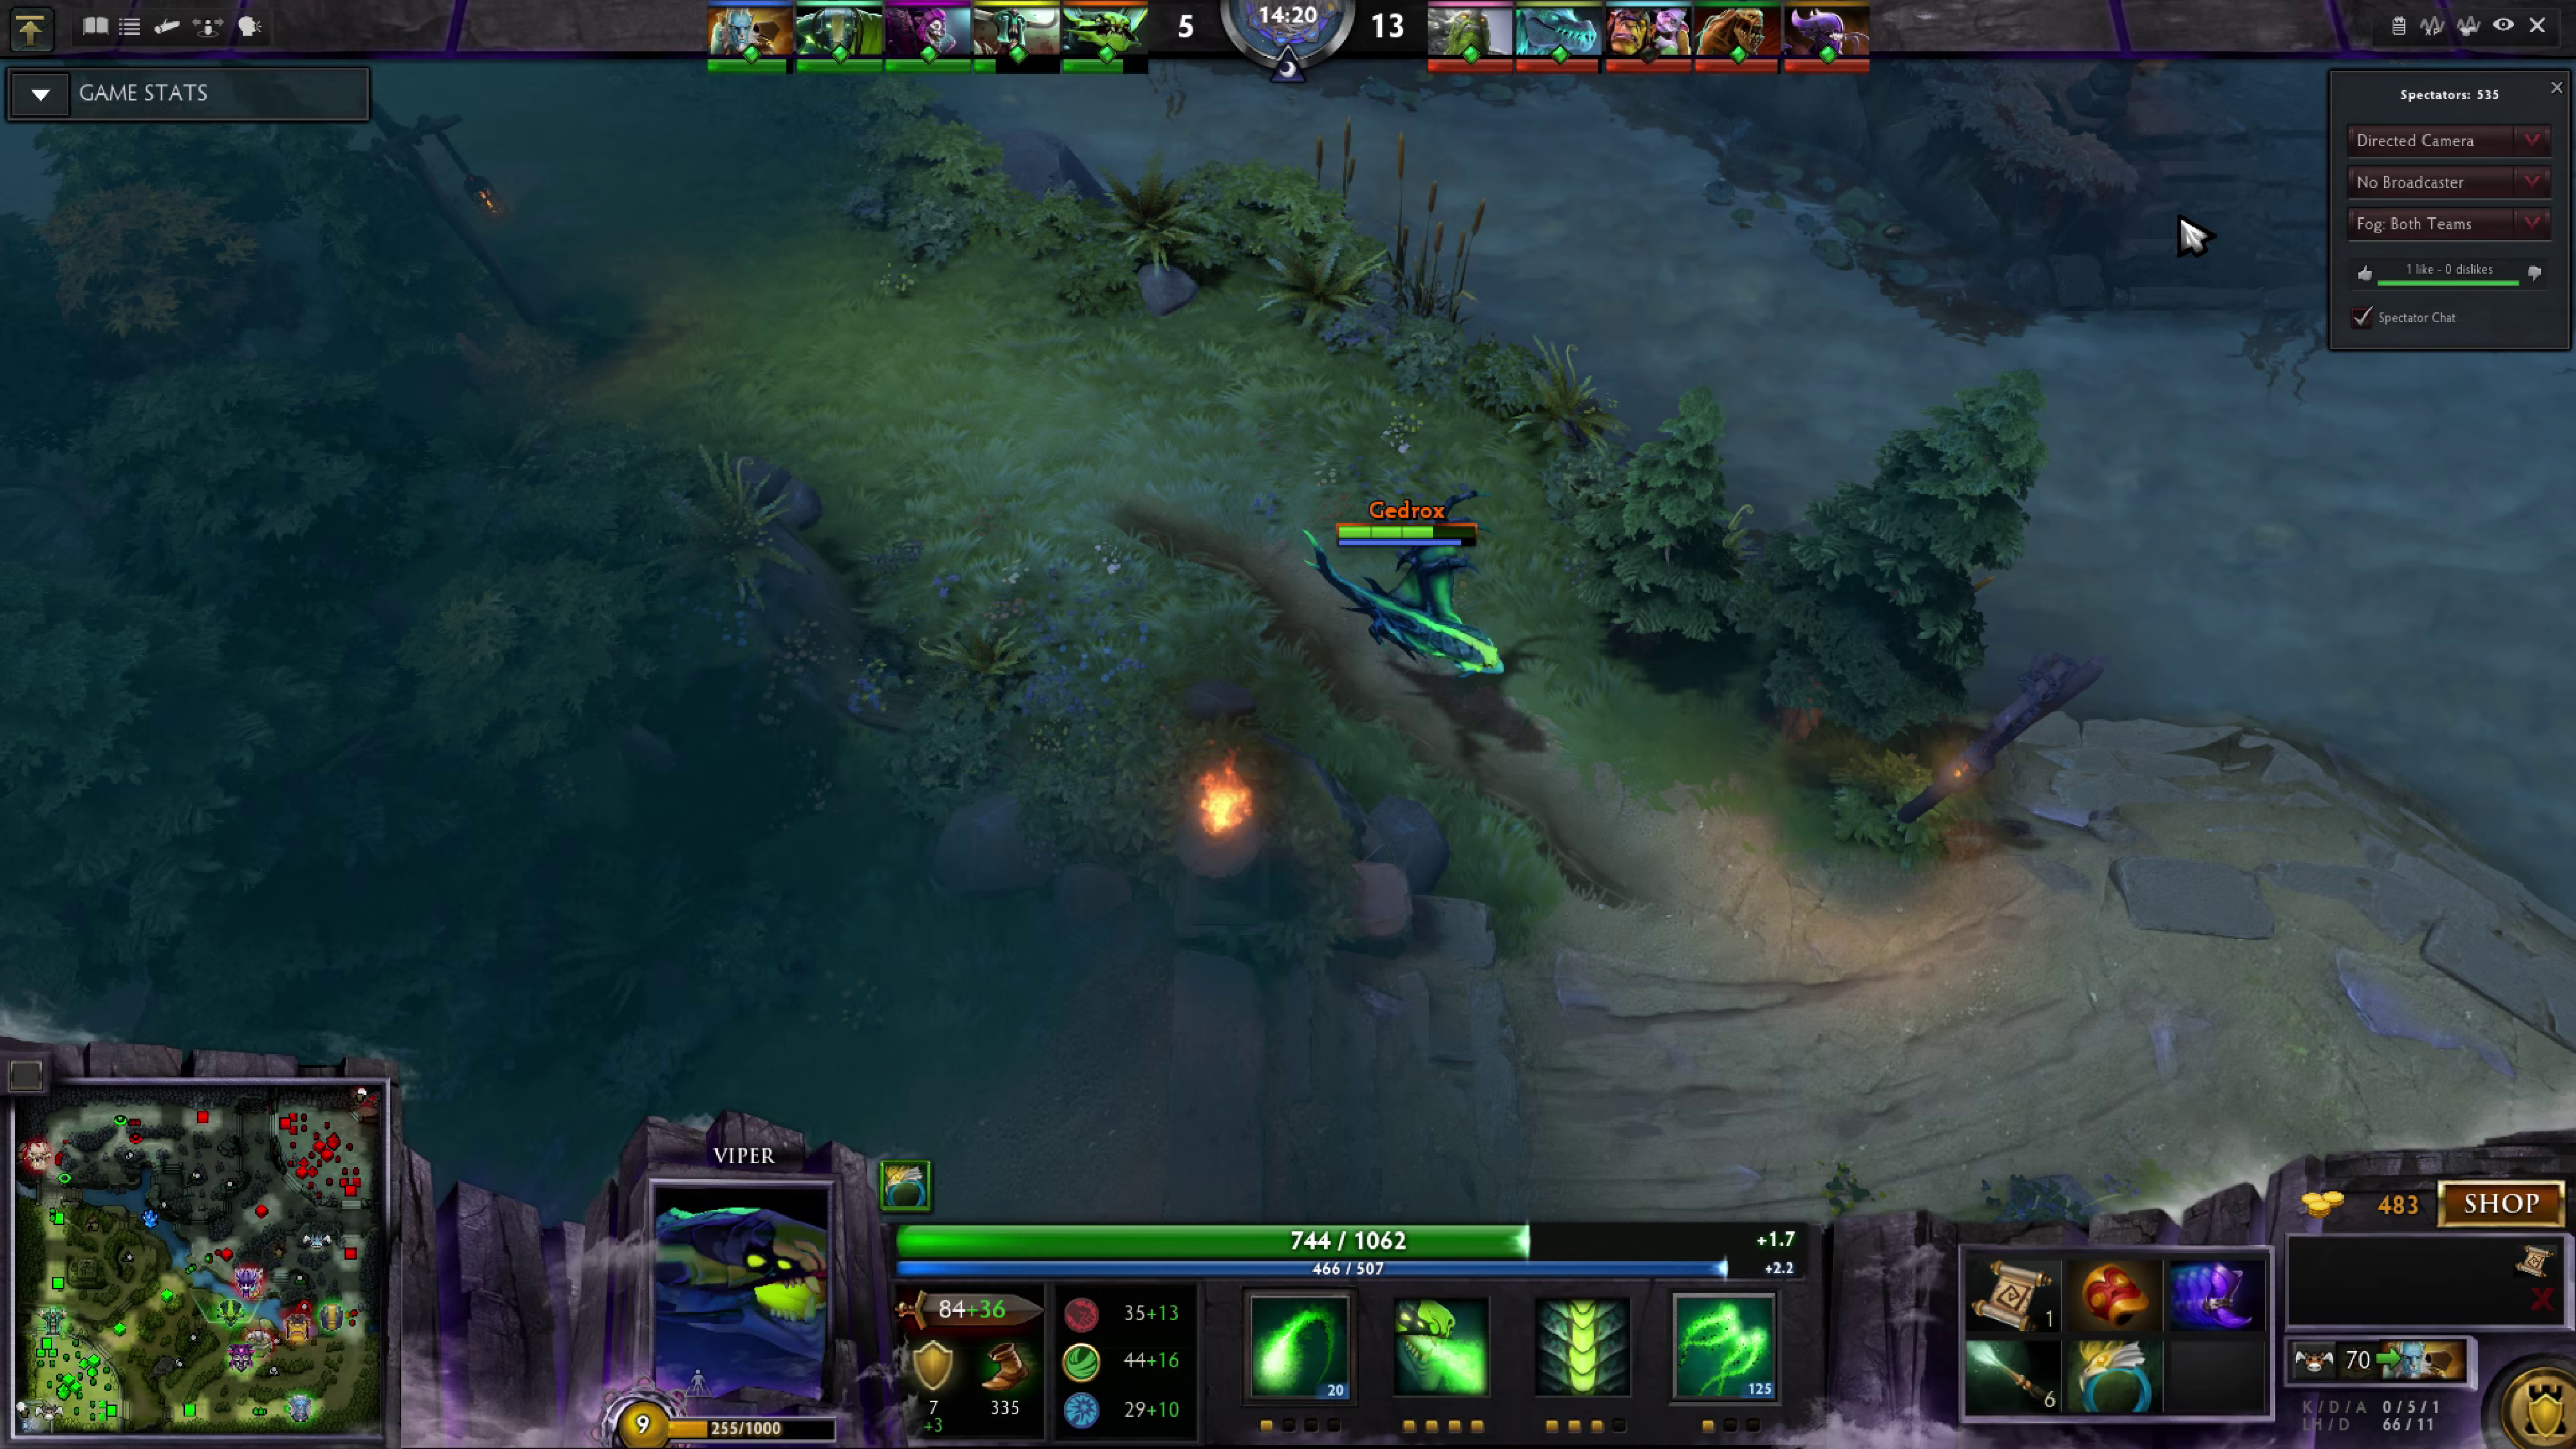
\includegraphics[width=0.885\textwidth]{dota2_jnd_decode.pdf}}
    \subcaptionbox{md-stage调整的JND优化快速算法解码图像\label{fig:dota2-md-dec}}
                    [\textwidth]{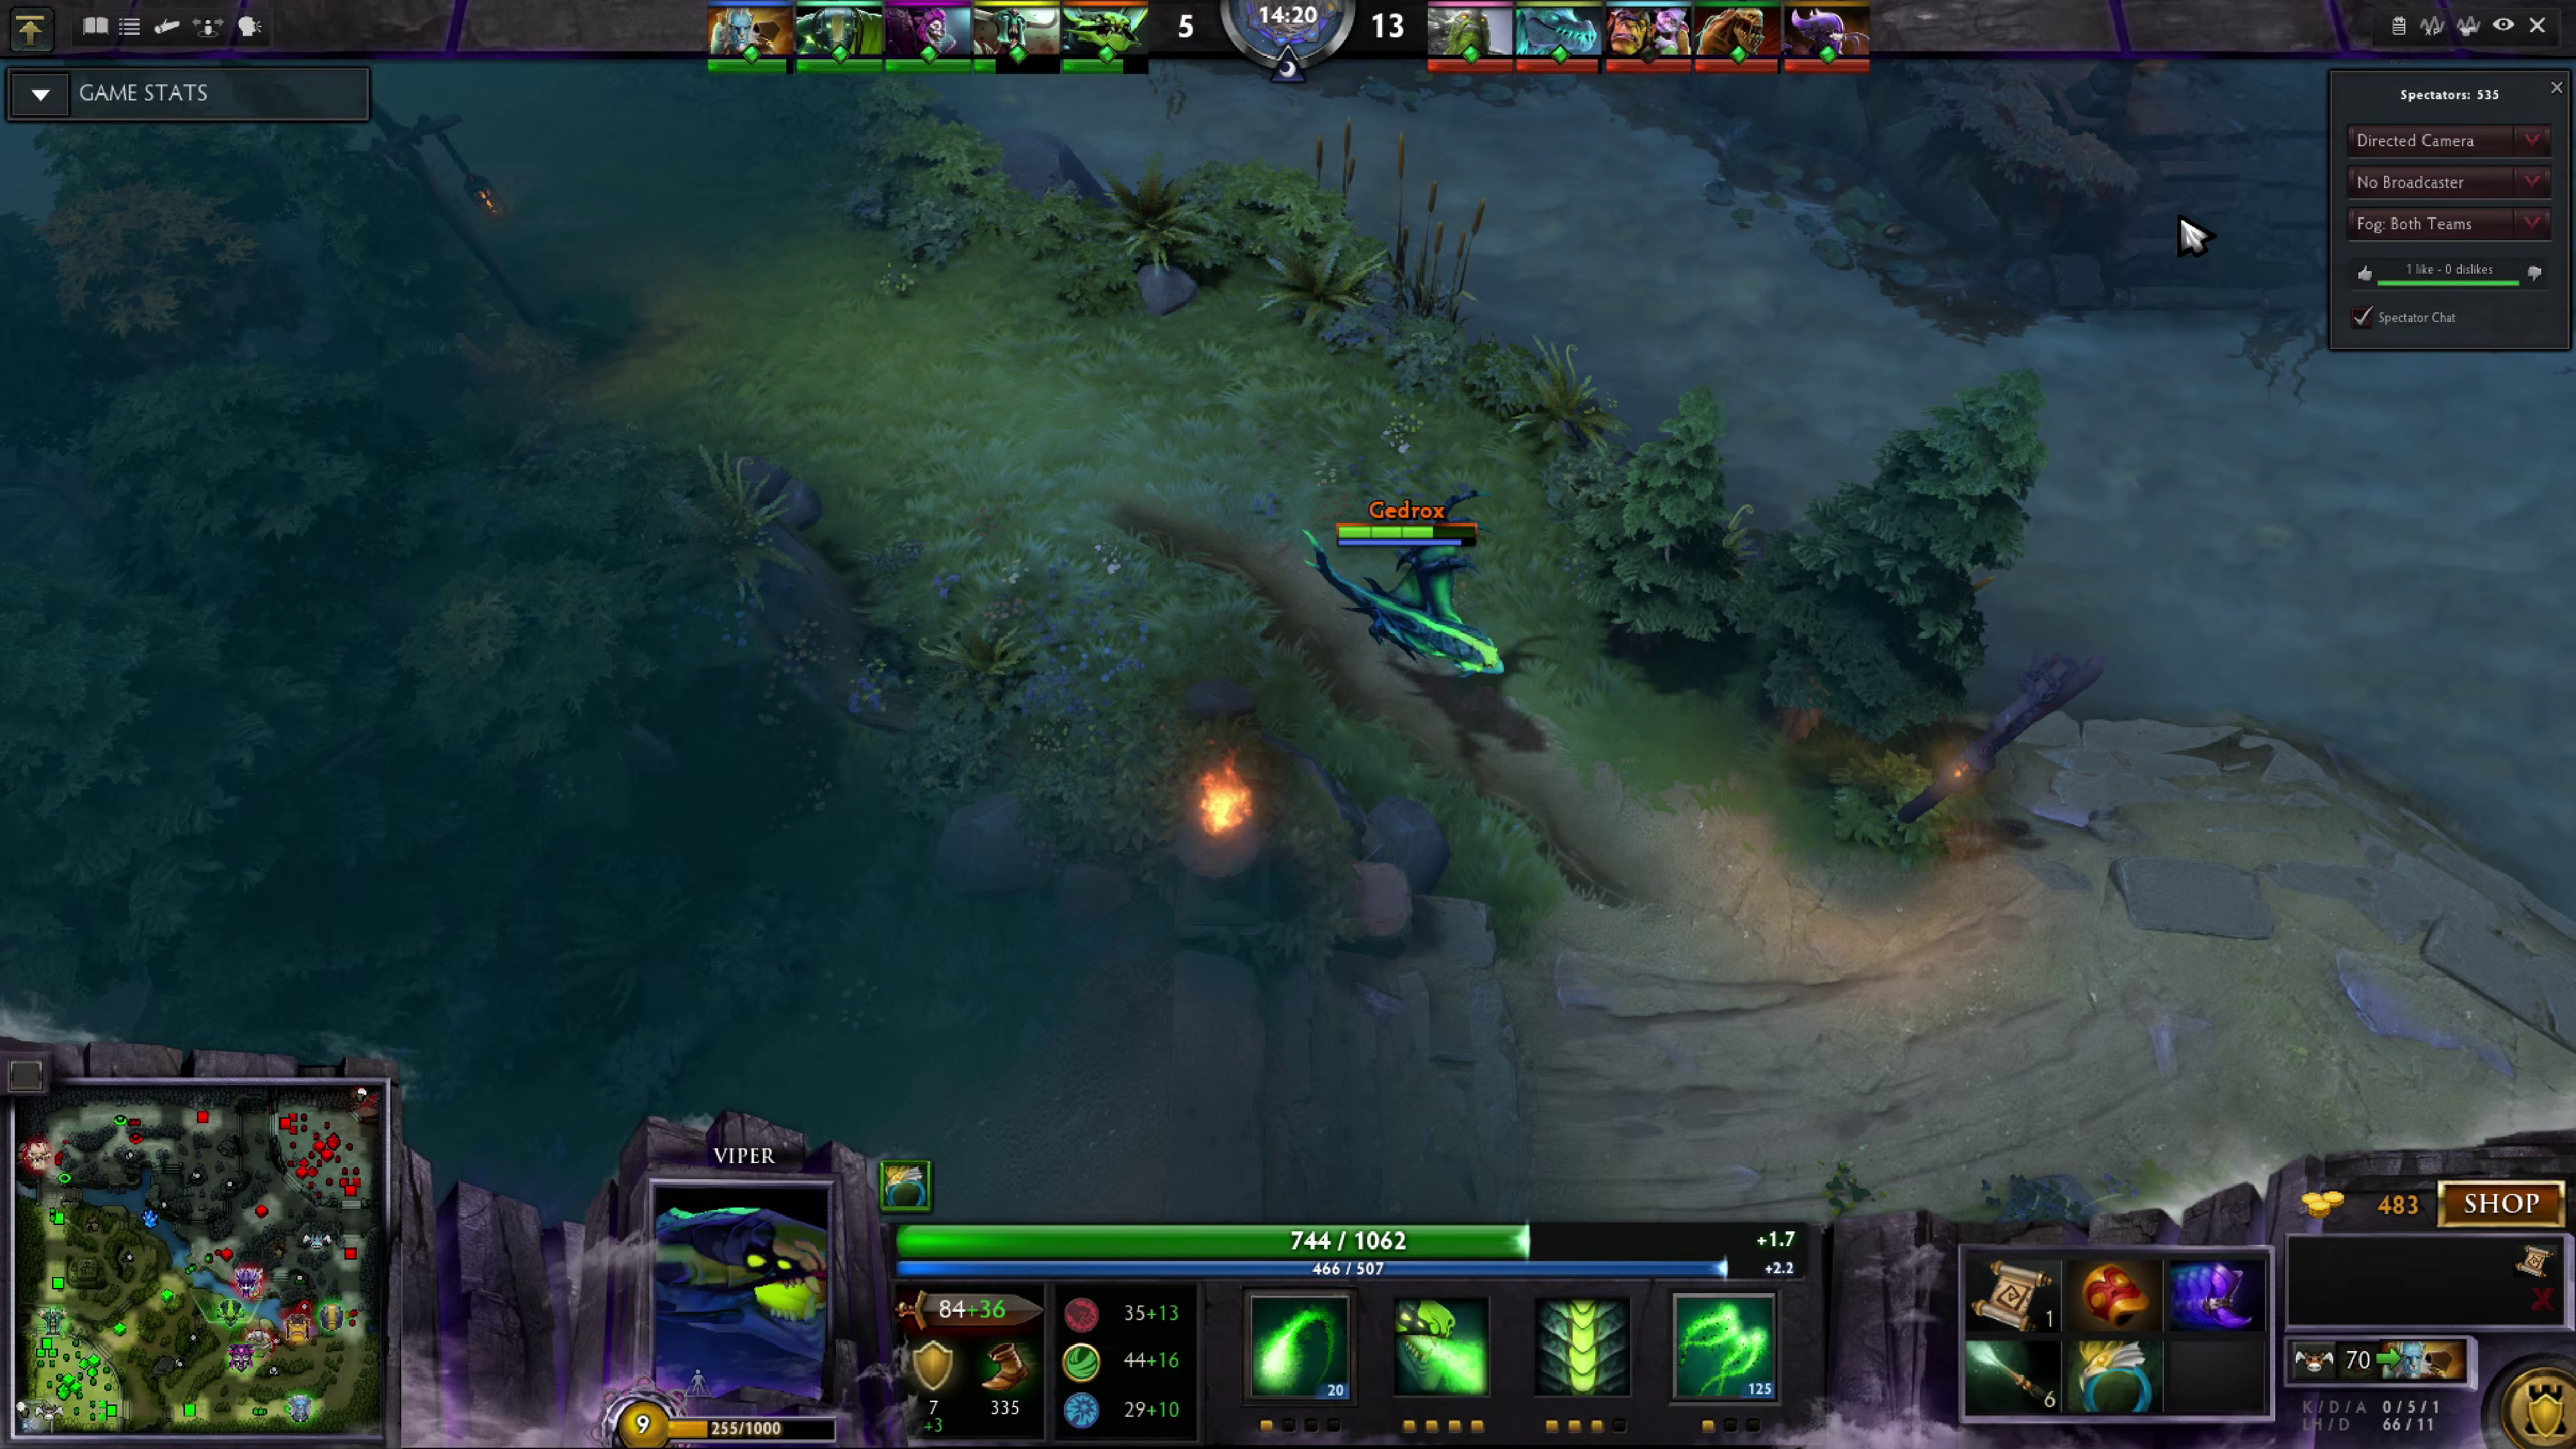
\includegraphics[width=0.885\textwidth]{dota2_md_dec.pdf}}
    \caption{原始算法与所提算法的解码对比图}
    \label{fig:dota2-decode}
  \end{figure}
\vspace{-10pt}
  \section{本章小结}

  本章提出了基于人眼感知特性的超级块快速划分算法。首先介绍了人眼视觉特性,包括亮度自适应性、视觉掩蔽效应和视觉注意机制,介绍了像素级JND模型的提出,以及根据像素级JND模型优化得到的块级JND模型。

  为进一步加速JND模型的计算,对背景亮度计算和亮度方差计算运用了SIMD方法进行加速,加速后只需1.7ms即可完成对一个1080p视频帧的JND模型计算。

  对JND感知阈值与AV1超级块划分结果进行统计分析,总结得到了与块划分相关的感知划分指标,并根据感知划分指标在twitch的游戏视频序列中的统计特性,分析确定了块划分提前终止划分的阈值。根据该阈值实现块划分时的提前终止,可以跳过大量的搜索过程,减少大量编码复杂度,降低编码时间。

  实验结果表明,在SVT-AV1的最快编码预设的基础上,在损失2\%左右编码性能的前提下,本章所提出的超级块快速划分算法在All Intra和Low Delay P两种GoP结构上均可以减少15\%左右的编码时间,进一步调整md-stage后可以在All Intra下减少30\%的编码时间。
